\documentclass[11pt]{article}
\usepackage[margin=1in]{geometry}
\usepackage{amsmath,amssymb,amsthm,mathtools}
\usepackage{booktabs,array,enumitem,xcolor,longtable,tikz-cd,graphicx,placeins}
\graphicspath{{atlas/figs/}}
\usepackage{xurl}
\usepackage[colorlinks=true,linkcolor=blue!50!black,citecolor=green!35!black,urlcolor=blue!50!black]{hyperref}
\usepackage[nameinlink]{cleveref}
\newtheorem{theorem}{Theorem}[section]
\newtheorem{proposition}[theorem]{Proposition}
\newtheorem{lemma}[theorem]{Lemma}
\newtheorem{corollary}[theorem]{Corollary}
\newtheorem{conjecture}[theorem]{Conjecture}
\theoremstyle{definition}
\newtheorem{definition}[theorem]{Definition}
\newtheorem{example}[theorem]{Example}
\newtheorem{remark}[theorem]{Remark}
\newtheorem{problem}[theorem]{Open problem}
\newcommand{\D}{\mathsf D}
\newcommand{\C}{\mathsf C}
\newcommand{\DT}{\mathsf D_{\mathbb T}}
\newcommand{\DK}{\mathsf D_{K}}
\newcommand{\T}{\mathbb T}
\newcommand{\R}{\mathbb R}
\newcommand{\Sh}{\mathsf{Sh}}
\newcommand{\Hyp}{\mathsf{Hyp}}
\newcommand{\ls}{\lambda^{\sigma}}
\newcommand{\lb}{\bar\lambda}
\newcommand{\id}{\mathrm{id}}
\newcommand{\cx}{\le_{\mathrm{cx}}}
\newcommand{\Law}{\operatorname{Law}}
\newcommand{\EE}{\mathbb E}
\newcommand{\PP}{\mathbb P}
\newcommand{\ebot}{e_{\perp}}
\newcommand{\etop}{e_{\top}}
\newcommand{\Pt}{\widetilde\Pi}
\newcommand{\rr}{\tilde r}
\newcommand{\val}{\operatorname{val}}
\newcommand{\trop}{\operatorname{trop}}
\newcommand{\Mix}{\operatorname{Mix}}
\newcommand{\Sec}{\operatorname{Sec}}
\newcommand{\an}{\mathrm{an}}
\newcommand{\Ctx}{\mathbf{Ctx}}
\newcommand{\Meas}{\mathbf{Meas}}
\newcommand{\E}{\mathsf E}
\crefname{problem}{open problem}{open problems}
\crefname{conjecture}{conjecture}{conjectures}
\title{\textbf{Shadows, Fibres and Secants of the Posterior Tower}\\[.4em]
\large Conditional expectations, Beck defects, and positive tropicalisation}
\author{Vinay K. Awasthi\\ Department of Applied Mathematics and Statistics, Johns Hopkins University}
\date{October 13, 2026}

\setlength{\emergencystretch}{3em}
\begin{document}
\maketitle

\begin{abstract}
The three-level posterior tower \cite{Tower} has two candidate mixed distributive laws, and both fail some Beck axioms. This paper
studies the failures through two operations on the tower's levels: \emph{pooling}, which replaces a law by conditional expectations of
it, and \emph{tropicalisation}, which replaces probabilities by their large-deviation rates. It unifies and corrects three earlier
manuscripts, on the Giry-monad formulation, on conditional shadows, and on fibres and secants. The changes are listed in
\cref{app:changes}.

\emph{Algebra.} For finite partitions $A,B$ of a full-support probability space, five conditions are equivalent:
\begin{itemize}
\item $E_AE_B=E_BE_A$;
\item $E_AE_B=E_{A\wedge B}$;
\item $A$ and $B$ are conditionally independent given the meet $A\wedge B$;
\item every connected component of the bipartite cell graph has a rank-one contingency block;
\item every singular value of the normalised contingency matrix is $0$ or $1$.
\end{itemize}
The identity $E_AE_B=E_{A\vee B}$ holds only when $A=B$. In general $(E_AE_B)^n\to E_{A\wedge B}$ at the exact rate $c^{2n-1}$, so
interchange holds laxly, through the meet.

\emph{Shadows.} A coherent context determines a star-shaped probability space centred at the level-one predictive. Shadows are
conditional expectations on this fixed space. They form a commutative band and satisfy interchange strictly. Shadows defined by
label maps on laws do not compose as conditional expectations.

\emph{Topology and order.} The barycentre has two continuous splittings, $\ebot=\eta\mu$ and $\etop=\D(\eta)\mu$. These form a
left-zero band and bound every barycentre fibre in convex order. A coherent context is a three-step simplex-valued martingale. The
shift law's level-one unit defect is the full convex-order diameter of a fibre; its multiplication defect is one
conditional-expectation step.

\emph{Categorical structure.} We construct the lifting functor from contexts to measure spaces in two versions and prove naturality of
the shadows along measure-preserving maps. The double category is the quintet construction of a locally preordered 2-category, in
which interchange is automatic. In this language each Beck defect computed so far is a single conditional-expectation step.

\emph{Geometry.} Over a real closed non-Archimedean field the valuation is a monad morphism to the min-plus distribution monad.
Classical barycentre fibres map onto tropical fibres. Positive mixtures map exactly onto tropical secants. The valuation factors
through the Berkovich analytification, and on positive points the square commutes. The Bayes posterior tropicalises to the hard
assignment, so the Voronoi walls of nearest-atom pooling are tropical walls. We also correct the Gaussian fusion square, the finite
stochastic-to-convex functor and the moment-variety programme.

\emph{Cohomology.} Conditional expectations are the restriction maps of the $L^2$ presheaf on the lattice of $\sigma$-algebras. Its
Beck--Chevalley condition is exactly conditional independence given the meet, with defect norm $c$. Compatible sections always glue in
finite dimensions, and gluing fails only when $c=1$. The Beck comparisons are restriction maps, never isomorphisms. Tropical fibres
are covered by assignment cells. The nerve computes their cohomology, and Farkas certificates of impossible assignment patterns, the
tropical form of the tower's lifting certificates, determine it. For Hardy--Weinberg mixtures the fibre has $b_0=2$ off the
collision locus and $b_0=1$ on it, with $b_1=0$, so the collision wall is a jump in $H^0$.

\emph{Hallucination.} In a three-token model observed through pairwise windows, a hallucination (an obstructed claim) is a failure of
gluing. It occurs below a straight wall in source-weight space, at agreement $\tfrac13$, and is certified by a Bell-type functional.
Above the wall, the two overlapping windows satisfy Beck--Chevalley iff the tokens are Markov through the shared token. The defect is
$c=|2\varepsilon-1|/(2\varepsilon)$ at the symmetric section. Tropicalisation sees only support-level hallucinations. A pre-registered test on public GPT-3.5 and GPT-4 answers finds that
cross-run disagreement detects wrong answers in all five tasks (AUROC $0.69$--$0.88$), and that the window defect exceeds its Markov null
in three of them. One worked example, the Hardy--Weinberg
atlas, illustrates every layer in seven figures generated by a script.

\emph{Places.} Read over the Berkovich spectrum $\mathcal{M}(\mathbb{Z})$, the context presheaf separates by place: the window data
always glue over $\mathbb{Q}$ and every $\mathbb{Q}_p$, Beck--Chevalley is decided at the trivial seminorm, and the hallucination
obstruction is supported at the archimedean place, the only one that carries order. A second study, on HaluEval with a local model,
finds that the disagreement detector adds information beyond answer length and that the within-sample windows fail Beck--Chevalley
through item-level difficulty. For three agents reporting towers about one state, convex order ranks their information (Blackwell), the
agent-level entropy term measures distance from a common prior, two overlapping pairs of logs always reconcile while three can fail
with a cycle certificate, and chain pooling is exact under Beck--Chevalley. Eight scripts check every finite claim (30, 8, 10, 9, 9, 4 and
6 checks, and 7 Monte Carlo checks of the statistical test), all passing. Code, figures and an interactive explorer are at
\url{https://github.com/vkawasth/Trainingless-Transformer-NoGradientDescent/tree/main/papers}.
\end{abstract}

\tableofcontents

%=====================================================================
\section{Introduction}
%=====================================================================

\subsection{The problem}
A three-level posterior tower records three things: a predictive $\rho\in\D X$, a law $\Pi\in\D^2X$ over predictives, and a law
$\Omega\in\D^3X$ over such laws. It also carries a shadow $\Sigma$ of labelled hypotheses. A candidate mixed distributive law on the
tower may fail some Beck axioms, and the failures are comparisons between constructions, not merely numerical discrepancies. The
motivating question is whether two ways of pooling information organise these comparisons, and whether the comparisons have a geometric
meaning. Three logically separate tasks are involved:
\begin{enumerate}[label=(\arabic*)]
\item define the pooling operators (shadows) and prove their operator identities;
\item build a category or double category in which the Beck comparisons are well-typed cells;
\item locate the comparisons geometrically: in barycentre fibres, in convex order, and after tropicalisation, in secant geometry.
\end{enumerate}
None of these implies another, and the paper keeps them apart.

\subsection{Guiding principles}
\begin{enumerate}[label=(\roman*)]
\item \emph{Compose operators on a fixed probability space.} Composing measure-valued maps that recompute their partitions after each
  step is a different operation. Most earlier difficulties came from mixing the two.
\item \emph{Conditional expectations interact through the meet, never the join.}
\item \emph{Probability tropicalises cleanly because it is positive.} Leading terms of positive series cannot cancel, so the
  valuation is a semiring homomorphism. Every geometric statement in the paper rests on this.
\end{enumerate}

\subsection{Main results}
\begin{enumerate}[label=(\Alph*)]
\item \textbf{Commutation} (\cref{thm:commute}): five equivalent conditions, a spectral and a combinatorial criterion among them.
  The join identity holds only for equal $\sigma$-algebras (\cref{prop:join}).
\item \textbf{Rate and lax interchange} (\cref{thm:rate,cor:lax}).
\item \textbf{Shadow algebra} (\cref{thm:band}): the canonical shadows of a context form a commutative band.
\item \textbf{Fibres and martingale} (\cref{prop:two-idempotents,prop:fibre,thm:martingale}).
\item \textbf{Beck defects located} (\cref{prop:beck-located,prop:single-step}).
\item \textbf{Lifting functor and naturality} (\cref{prop:functor-component,prop:functor-base,prop:naturality}); quintet double
  category (\cref{prop:quintets}).
\item \textbf{Tropical tower} (\cref{thm:monad}), \textbf{fibre lifting} (\cref{thm:lift}), \textbf{tropical secants}
  (\cref{thm:secant}) and the \textbf{Berkovich square} (\cref{thm:berk}).
\item \textbf{Zero-temperature shadows and walls} (\cref{prop:posterior,prop:walls}).
\item \textbf{Cohomology}: Beck--Chevalley for the $L^2$ presheaf is conditional independence (\cref{thm:bc}); gluing and the
  degree-one obstruction (\cref{thm:gluing}); fibre cohomology from the nerve and its certificates (\cref{thm:nerve}); the
  Hardy--Weinberg computation (\cref{thm:hw-topology}).
\item \textbf{Hallucination}: a three-token model in which hallucination is a gluing failure with a certificate
  (\cref{prop:three-bit}), and the window shadows' Beck--Chevalley defect measures non-Markov coupling (\cref{prop:windows}); its
  tropical shadow is support-level only (\cref{prop:halluc-trop}).
\end{enumerate}

\subsection{Status}
\begin{center}\small
\begin{tabular}{>{\raggedright}p{9cm}>{\raggedright\arraybackslash}p{5.2cm}}\toprule
Statement & Status\\\midrule
operator commutation, rate, lax interchange & proved, finite and general\\
canonical shadows, band, naturality & proved\\
fibres, martingale, location of the (U) and (M) defects & proved\\
lifting functor, quintet double category & proved\\
a 2-category in which $\D$, $\C_3$ and the laws act monotonically & open (\cref{op:twocat})\\
tropical tower, fibre lifting, tropical secants, Berkovich square & proved\\
tropical identifiability inside a model & open (\cref{op:ident})\\
wall-crossing formula for Gaussian mixture towers & proposed (\cref{conj:wall})\\
$L^2$ presheaf: Beck--Chevalley, gluing, comparisons are restrictions & proved\\
fibre cohomology via assignment-cell nerves; certificates determine it & proved; Hardy--Weinberg computed\\
lifting obstructions inside a model as cohomology classes & open (\cref{op:cech})\\
three-token hallucination: gluing failure, window Beck--Chevalley, tropical shadow & proved\\
window defect on real model outputs (pre-registered Study 1) & nonzero in 3 of 5 tasks\\
obstruction below $\tfrac13$ in pairwise-elicited model answers & kit ready (Study 3); needs model access\\
\bottomrule
\end{tabular}
\end{center}

\subsection{Conventions}
$X$ and $B$ denote finite sets, and $\D$ is the finite distribution monad with $\eta_X(x)=\delta_x$ and $\mu_X(\Pi)=\sum_\rho\Pi(\rho)\rho$.
We identify $\D B$ with the simplex $\Delta_B\subset\R^B$, with the $\ell^1$ metric. A \emph{finite probability space} $(I,p)$ has
$p(i)>0$ for all $i$, and its $\sigma$-algebras are partitions. For a partition $A$, $E_A$ is conditional expectation, acting
coordinatewise on $\R^X$-valued functions: $(E_AZ)(i)=\sum_{j\in A(i)}p(j)Z(j)/p(A(i))$, where $A(i)$ is the cell of $i$. In the
tower paper \cite{Tower}, the letters $L$ and $R$ also denote the two sides of the (Cm) diagram. Here $L_c$ and $R_c$ always denote
shadows (\cref{def:shadows}).

%=====================================================================
\section{The posterior tower}\label{sec:tower}
%=====================================================================

\subsection{Levels and contexts}
For a finite set $B$, the iterated distribution spaces $\D B,\D^2B,\D^3B,\dots$ carry barycentre maps satisfying the monad laws. A
hypothesis is $h=(\theta,r)\in\Hyp B=\Theta\times\D B$, with predictive $q(h)=r$. $\Hyp$ is a functor and $q$ is natural
\cite[Def.~3.1]{Tower}. The shadow space is $\Sh(B)=\D(\Hyp B)$. A context is $c=(\rho,\Pi,\Omega,\Sigma)$ with $\rho\in\D B$,
$\Pi\in\D^2B$, $\Omega\in\D^3B$ and $\Sigma\in\Sh B$.

\begin{definition}[Coherent context]\label{def:coherent}
$c$ is \emph{coherent} if
\begin{equation}\label{eq:coherent}
\mu(\Pi)=\rho,\qquad\mu(\Omega)=\Pi,\qquad\D(q)(\Sigma)=\Pi .
\end{equation}
\end{definition}

\begin{remark}[Typing]
The third condition is meaningful because $q$ lands in $\D B$, the underlying space of $\Pi$. Any variant of the shadow component must
come with its own projection to $\D B$ and its action on maps $f\colon B\to B'$. For $\Hyp=\Theta\times\D(-)$ this action is
$\Hyp(f)(\theta,r)=(\theta,f_*r)$.
\end{remark}

\subsection{The absolute tower and the two laws}
The absolute tower $\C_3X=X\times\D X\times\D^2X\times\D^3X\times\Sh X$ is a comonad, with comultiplication
$\delta(x,c)=((x,c),\E_3(j_c)(c))$, where $j_c(y)=(y,c)$ \cite[\S6]{Tower}. Applying it at $\D X$ gives
$\C_3(\D X)=\D X\times\D^2X\times\D^3X\times\D^4X\times\Sh(\D X)$. For a sample $M=\sum_ia_i\delta_{(x_i,c_i)}$:
\begin{itemize}
\item the \emph{shift law} $\ls$ keeps each sample's context entries, moving them one level up;
\item the \emph{averaging law} $\lb$ pushes contexts through the unit and averages them.
\end{itemize}

\subsection{Beck axioms}
A mixed distributive law $\lambda\colon\D\C\Rightarrow\C\D$ must satisfy the unit (U), counit (Co), multiplication (M) and
comultiplication (Cm) diagrams \cite[Def.~2.1]{Tower}. The shift law satisfies (Co) and fails (U), (M) and (Cm). The averaging law
satisfies (U), (Co) and (M) and fails (Cm) \cite[Thms.~8.3, 8.6, 8.7]{Tower}. The base-relative tower has a strict law
\cite[Thm.~9.8]{Tower}. A failure produces two parallel composites with the same source and target, and the comparison between them
is the \emph{Beck defect}.

%=====================================================================
\section{Algebra of conditional expectations}\label{sec:algebra}
%=====================================================================

\subsection{The partition lattice}
Partitions of $I$ form a lattice under refinement. The \emph{join} $A\vee B$ has cells $a\cap b$. The \emph{meet} $A\wedge B$ is the
finest common coarsening. As $\sigma$-algebras, $A\vee B=\sigma(A\cup B)$ and $A\wedge B=A\cap B$.

\begin{lemma}[The meet is $\pi_0$ of a bipartite graph]\label{lem:meet}
Let $G(A,B)$ be the bipartite graph on the cells of $A$ and of $B$, with an edge $a$--$b$ whenever $a\cap b\ne\emptyset$. The cells of
$A\wedge B$ are the unions over the connected components of $G(A,B)$, and $L^2(A)\cap L^2(B)=L^2(A\wedge B)$.
\end{lemma}
\begin{proof}
A set lies in $A\cap B$ iff it is a union of $A$-cells and a union of $B$-cells, i.e.\ iff it is closed under the edge relation. A
function lies in $L^2(A)\cap L^2(B)$ iff it is constant on cells of both partitions, i.e.\ iff it is constant on components.
\end{proof}

\subsection{The commutation theorem}
Write $N_{ab}=p(a\cap b)$ for the contingency matrix and $K=D_A^{-1/2}ND_B^{-1/2}$, with $D_A=\mathrm{diag}(p(a))$ and
$D_B=\mathrm{diag}(p(b))$.

\begin{lemma}[A sufficient pair]\label{lem:smallC}
On any probability space, let $C\subseteq A\cap B$ be sub-$\sigma$-algebras such that $A$ and $B$ are conditionally independent given
$C$. Then $E_AE_B=E_C=E_BE_A$, and $C=A\cap B$ up to null sets.
\end{lemma}
\begin{proof}
For $V\in L^2(B)$ and $U\in L^2(A)$, conditional independence gives
$\EE[UV]=\EE[\EE[U\mid C]\EE[V\mid C]]=\EE[U\,\EE[V\mid C]]$, using $C\subseteq A$. So $E_AV=E_CV$, and hence $E_AE_B=E_CE_B=E_C$,
using $C\subseteq B$. The other order is symmetric. The range of $E_C$ is $L^2(C)$, and that of the commuting product is
$L^2(A)\cap L^2(B)=L^2(A\cap B)$.
\end{proof}

\begin{theorem}[Commutation]\label{thm:commute}
For partitions $A,B$ of a finite probability space the following are equivalent:
\begin{enumerate}[label=(\roman*)]
\item $E_AE_B=E_BE_A$;
\item $E_AE_B=E_{A\wedge B}$;
\item $A$ and $B$ are conditionally independent given $A\wedge B$;
\item on each component $\gamma$ of $G(A,B)$, the block $N|_\gamma$ has rank one, i.e.\ $p(a\cap b)p(\gamma)=p(a)p(b)$ for all cells
  $a,b\subseteq\gamma$;
\item every singular value of $K$ is $0$ or $1$.
\end{enumerate}
The equivalences (i)$\Leftrightarrow$(ii)$\Leftrightarrow$(iii) hold on every probability space, with $A\wedge B$ read as $A\cap B$.
The value $1$ in (v) has multiplicity equal to the number of components. Nestedness ($A\subseteq B$ or $B\subseteq A$) implies (iv).
\end{theorem}
\begin{proof}
(iii)$\Rightarrow$(ii) is \cref{lem:smallC}. (ii)$\Rightarrow$(i): $E_{A\wedge B}$ is self-adjoint, so
$E_BE_A=(E_AE_B)^*=E_AE_B$. (i)$\Rightarrow$(ii): the product of commuting orthogonal projections is the projection onto the
intersection of their ranges, which is $L^2(A\wedge B)$ by \cref{lem:meet}. (ii)$\Rightarrow$(iii): with $C=A\wedge B$,
$\EE[UV\mid C]=\EE[U\,E_AV\mid C]=\EE[U\,E_CV\mid C]=E_CU\cdot E_CV$, since $E_AV=E_AE_BV=E_CV$ is $C$-measurable.

(iii)$\Leftrightarrow$(iv): on a finite space it suffices to test indicators. Cells lie inside single components, so conditional
independence given $C$ reads $p(a\cap b\mid\gamma)=p(a\mid\gamma)p(b\mid\gamma)$. This says $N|_\gamma$ is the outer product of its
margins divided by its total, which for a nonnegative matrix is the same as rank one.

(ii)$\Leftrightarrow$(v): in the orthonormal bases $1_a/\sqrt{p(a)}$ and $1_b/\sqrt{p(b)}$, $E_A|_{L^2(B)}$ has matrix $K$, whose
singular values are the cosines of the principal angles between $L^2(A)$ and $L^2(B)$. The value $1$ occurs exactly on
$L^2(A\wedge B)$. Condition (ii) holds iff all other angles are $\pi/2$. If $A\subseteq B$, every $A$-cell is a component and (iv) is
trivial.
\end{proof}

Check A1 confirms the five-way equivalence on 600 random instances, 449 commuting and 151 not.

\begin{proposition}[The join identity]\label{prop:join}
$E_AE_B=E_{A\vee B}$ holds iff $A=B$ up to null sets.
\end{proposition}
\begin{proof}
The range of $E_AE_B$ lies in $L^2(A)$. If it equals $L^2(A\vee B)\supseteq L^2(B)$, then $B\subseteq A$, so $E_AE_B=E_B$ and
$E_{A\vee B}=E_A$, whence $A=B$.
\end{proof}

\begin{example}[A non-commuting pair]\label{ex:46}
Let $I=\{1,2,3,4\}$ with $p=(\tfrac38,\tfrac18,\tfrac18,\tfrac38)$, $Z(i)=i$, $A_L=\{\{1,2\},\{3,4\}\}$ and $A_R=\{\{1,3\},\{2,4\}\}$. Then
\[
(E_{A_R}E_{A_L}Z)(1)=\tfrac34\cdot\tfrac54+\tfrac14\cdot\tfrac{15}4=\tfrac{15}8,\qquad(E_{A_L}E_{A_R}Z)(1)=\tfrac34\cdot\tfrac32+\tfrac14\cdot\tfrac72=2 .
\]
$G(A_L,A_R)$ is a 4-cycle, so the meet is trivial. The block
$N=\begin{psmallmatrix}3/8&1/8\\1/8&3/8\end{psmallmatrix}$ has rank two, and $K$ has singular values $1$ and $\tfrac12$ (check A3).
\end{example}

\subsection{Worked regimes}
\begin{itemize}
\item \emph{Committed} ($A=B$): the operators coincide. This is a consistency check only.
\item \emph{Inherited} ($A\subseteq B$ or $B\subseteq A$): the operators commute with product the coarser one.
\item \emph{General}: commutation holds iff (iv) of \cref{thm:commute} holds. Adding labels does not by itself produce conditional
  independence. \Cref{ex:46} shows the generic outcome.
\end{itemize}

\subsection{The general case: rate and lax interchange}

\begin{theorem}[Alternating projections, exact rate]\label{thm:rate}
Let $c$ be the cosine of the Friedrichs angle between $L^2(A)$ and $L^2(B)$. In the finite case, $c$ is the largest singular value of
$K$ strictly below $1$, or $0$ if there is none. Then
\[
\lVert(E_AE_B)^n-E_{A\wedge B}\rVert=c^{2n-1}\qquad(n\ge1).
\]
On a general probability space the identity holds with the Friedrichs cosine. Then $c<1$ iff $L^2(A)+L^2(B)$ is closed. Otherwise
$(E_AE_B)^n\to E_{A\wedge B}$ only strongly, and the convergence can be arbitrarily slow.
\end{theorem}
\begin{proof}
The identity is the Kayalar--Weinert theorem \cite{KayalarWeinert1988}, with $L^2(A)\cap L^2(B)=L^2(A\wedge B)$. Strong convergence
is von Neumann's theorem \cite{vonNeumann1950}, and arbitrarily slow convergence is in \cite{BauschkeDeutschHundal2009}.
\end{proof}

Check A4 verifies the rate to $10^{-9}$ for $n\le6$ on 157 non-commuting pairs.

\begin{definition}[Convex order]
For finitely supported laws $Q,Q'$ on a convex set, $Q\cx Q'$ if $\int\varphi\,dQ\le\int\varphi\,dQ'$ for all convex $\varphi$. By
Strassen's theorem \cite{Strassen1965} this holds iff $Q=\Law(\EE[U'\mid G])$ for some $U'\sim Q'$ and some sub-$\sigma$-algebra $G$.
\end{definition}

\begin{corollary}[Lax interchange]\label{cor:lax}
$E_{A\wedge B}E_AE_B=E_{A\wedge B}=E_{A\wedge B}E_BE_A$. Hence
\[
\Law(E_{A\wedge B}Z)\cx\Law(E_AE_BZ)\cx\Law(E_BZ)\cx\Law(Z),
\]
and symmetrically through $E_BE_AZ$. The laws $\Law((E_AE_B)^nZ)$ decrease in convex order, and
\[
W_2\big(\Law((E_AE_B)^nZ),\Law(E_{A\wedge B}Z)\big)\le c^{2n-1}\lVert Z-E_{A\wedge B}Z\rVert_{L^2(p)} .
\]
\end{corollary}
\begin{proof}
The tower property gives the first identity. Each displayed law is that of a conditional expectation of the next on the same space.
For the rate, $(E_AE_B)^n-E_{A\wedge B}=((E_AE_B)^n-E_{A\wedge B})(I-E_{A\wedge B})$; apply \cref{thm:rate} and use the identity
coupling to bound $W_2$.
\end{proof}

So without nestedness or conditional independence, interchange does not hold strictly. It holds through the cospan
$E_AE_B\Rightarrow E_{A\wedge B}\Leftarrow E_BE_A$ of convex-order comparisons. These are identities exactly under \cref{thm:commute},
and they shrink at the rate of \cref{thm:rate}.

\subsection{Conditioning on a third variable}
\begin{proposition}\label{prop:gauss}
Let $X_L\perp X_R\mid H$ on a finite space with full support. Then:
\begin{enumerate}[label=(\alph*)]
\item $E_{\sigma(X_L,H)}E_{\sigma(X_R,H)}=E_{\sigma(H)}=E_{\sigma(X_R,H)}E_{\sigma(X_L,H)}$;
\item $E_{\sigma(X_L)}$ and $E_{\sigma(X_R)}$ commute iff $X_L\perp X_R$ marginally. With full support the meet is trivial, so this
  fails as soon as both channels depend on $H$.
\end{enumerate}
\end{proposition}
\begin{proof}
(a) is \cref{lem:smallC} with $C=\sigma(H)$. (b) With full support, $G(\sigma(X_L),\sigma(X_R))$ is complete bipartite, hence
connected; apply \cref{thm:commute}.
\end{proof}

Conditional independence given a third variable is therefore not a commutation hypothesis. The conditioning variable must be built
into both $\sigma$-algebras (check A7).

%=====================================================================
\section{Shadows}\label{sec:shadows}
%=====================================================================

\subsection{Label-defined shadows on laws}
Let $S=\D B$ with its Borel $\sigma$-algebra, and let $a\colon S\to I_a$ be a measurable \emph{label map} with finite codomain. For
$\nu\in\D(S)$ with identity variable $Z$, put $m_a=\EE_\nu[Z\mid\sigma(a)]$ and define the label shadow $P_a(\nu)=(m_a)_*\nu$.

\begin{proposition}[Properties of a single label shadow]\label{prop:label-props}
\begin{enumerate}[label=(\alph*)]
\item $\int\rho\,dP_a(\nu)=\int\rho\,d\nu$, and $P_a(\nu)\cx\nu$.
\item If $a(m_a(\rho))=a(\rho)$ for $\nu$-a.e.\ $\rho$ (\emph{label preservation}), then $P_a(P_a\nu)=P_a\nu$. Without label
  preservation, the first barycentre can move a point into another label class, and idempotence can fail.
\end{enumerate}
\end{proposition}
\begin{proof}
(a) is the tower property together with Strassen's theorem. (b) Write $Y=m_a(Z)$. Then $Y$ is $\sigma(a(Z))$-measurable, and label
preservation gives $a(Y)=a(Z)$, so $\EE[Y\mid a(Y)]=Y$.
\end{proof}

\begin{proposition}[Composites of label shadows are single poolings]\label{prop:naive}
For label maps $a,b$,
\[
P_b(P_a(\nu))=\Law\big(E_{A'}Z\big),\qquad A'=\sigma(b\circ m_a)\subseteq\sigma(a).
\]
So $P_bP_a$ pools once, onto a coarsening of the \emph{first} partition. The equation $P_bP_a=P_aP_b$ compares coarsenings of two
different partitions. It is not the operator identity $E_AE_B=E_BE_A$, and \cref{thm:commute} does not govern it.
\end{proposition}
\begin{proof}
$m_a$ is constant on $\sigma(a)$-cells, so $b\circ m_a$ is too. Pooling the atoms of $P_a\nu$ along $b$ merges whole cells, and a
barycentre of barycentres is the barycentre of the union.
\end{proof}

\begin{example}[Threshold labels]\label{ex:threshold}
On $\D\{0,1\}\cong[0,1]$, let $\nu$ be uniform on $\{0.1,0.3,0.7,0.9\}$, $a=[s\ge\tfrac12]$ and $b=[s\ge\tfrac14]$. Then
$P_b(P_a\nu)=\tfrac12\delta_{0.2}+\tfrac12\delta_{0.8}$, whereas $P_a(P_b\nu)=\tfrac14\delta_{0.1}+\tfrac34\delta_{19/30}$. The
fixed-space operators also fail to commute, but with different values (checks C2, C3).
\end{example}

\subsection{Labelled random measures}
\begin{definition}\label{def:lrm}
A \emph{labelled random measure} over $X$ is a triple $(I,p,Z)$: a finite probability space and a map $Z\colon I\to\D X$. A
morphism $f\colon(I,p,Z)\to(I',p',Z')$ is a map with $f_*p=p'$ and $Z'\circ f=Z$. The functor $\Law(I,p,Z)=Z_*p\in\D^2X$ forgets the
labels.
\end{definition}

\begin{proposition}[Shadows on a fixed space]\label{prop:law-functor}
For partitions $A,B$ of $I$:
\begin{enumerate}[label=(\alph*)]
\item $E_A$ is idempotent, preserves $\EE Z$, and satisfies $\Law(E_AZ)\cx\Law(Z)$;
\item composition of shadows is composition of conditional expectations;
\item $\Law(E_AE_BZ)=\Law(E_BE_AZ)$ for all $Z$ iff (i)--(v) of \cref{thm:commute} hold (when $|X|\ge2$).
\end{enumerate}
\end{proposition}
\begin{proof}
(a) and (b) are immediate. For ``only if'' in (c): the energy $\int\lVert v\rVert^2\,d\Law(\cdot)$ is a function of the law. Write
$Z=\rho_0+Y$ with $\rho_0$ in the relative interior and $Y$ small with zero coordinate sums. Then
$\lVert E_AE_BY\rVert=\lVert E_BE_AY\rVert$ on an open set, hence everywhere, and polarisation gives $S:=E_BE_AE_B=E_AE_BE_A$. The
range of $S$ lies in $L^2(M)$ with $M=A\wedge B$, and $S$ is self-adjoint, so $S=E_MSE_M=E_M$. For $Y\in L^2(B)$ this reads
$\lVert E_AY\rVert=\lVert E_MY\rVert$, so $E_AY=E_MY$ by Pythagoras, which is (ii).
\end{proof}

\begin{proposition}[Naturality]\label{prop:naturality}
Let $f\colon(I,p)\to(I',p')$ be measure preserving, and let $A=f^{-1}A'$, $B=f^{-1}B'$. Then $E_A(Z'\circ f)=(E_{A'}Z')\circ f$, and
likewise for $B$.
\end{proposition}
\begin{proof}
$f^{-1}(a')$ is a cell of $A$ of mass $p'(a')$, and the average of $Z'\circ f$ over it is the average of $Z'$ over $a'$ (check G2).
\end{proof}

\subsection{The star space of a context and the canonical shadows}
\begin{definition}[Star space]\label{def:star}
For a coherent context $c$, let $\kappa(\theta\mid r)=\Sigma(\theta,r)/\Pi(r)$. The \emph{star space} of $c$ has points
$(\Pt,r,\theta,x)$ with weights
\[
p_c(\Pt,r,\theta,x)=\Omega(\Pt)\,\Pt(r)\,\kappa(\theta\mid r)\,r(x),
\]
restricted to positive weights. Write $\rr$ for the coordinate $r$ and $Z=\delta_x$.
\end{definition}

Given $\rr$, the three \emph{leaves} $\Pt$, $\theta$ and $x$ are independent. The marginals recover the context:
$\Law(\Pt)=\Omega$, $\Law(\rr)=\Pi$, $\Law(\theta,\rr)=\Sigma$ and $\Law(x)=\rho$ (check B1). The context itself does not couple $\Omega$
with $\Sigma$; the conditional product over $\rr$ is the canonical coupling.

\begin{definition}[Canonical shadows]\label{def:shadows}
For a set $T\subseteq\{\mathrm{lev2},\mathrm{hyp},\mathrm{obs}\}$ of leaves, let
\[
G_T=\sigma(\rr,\ \text{leaves in }T),\qquad S_T=E_{G_T}.
\]
The \emph{left shadow} is $L_c=S_{\{\mathrm{lev2}\}}$ and the \emph{right shadow} is $R_c=S_{\{\mathrm{hyp}\}}$.
\end{definition}

\begin{theorem}[The shadow algebra is a commutative band]\label{thm:band}
$S_TS_U=S_{T\cap U}=S_US_T$ for all leaf sets $T,U$. In particular $L_cR_c=R_cL_c=E_{\sigma(\rr)}$.
\end{theorem}
\begin{proof}
$G_{T\cap U}\subseteq G_T\cap G_U$. The leaves in $T\setminus U$ and in $U\setminus T$ are independent given $\rr$ and the leaves in
$T\cap U$, so \cref{lem:smallC} applies.
\end{proof}

Check B2 verifies all $8\times8$ products on 60 random coherent contexts. The homomorphism $T\mapsto S_T$ need not be injective: if
$\theta$ is a function of $\rr$, then $R_c=S_\emptyset$.

\begin{proposition}[Dropping the centre]\label{prop:no-centre}
The label-only shadows $E_{\sigma(\Pt)}$ and $E_{\sigma(\theta)}$ commute iff \cref{thm:commute} holds for them. They fail to commute in
40 of 60 random contexts (check B3).
\end{proposition}

\begin{proposition}[Markov absorption]\label{prop:absorb}
For $Z=\delta_x$: (a) $R_cZ=E_{\sigma(\rr)}Z=\rr$; (b) $E_{\sigma(\theta)}Z=\sum_r\Sigma(r\mid\theta)\,r$, and in general
$E_{\sigma(\rr)}E_{\sigma(\theta)}Z\ne E_{\sigma(\theta)}Z$ (59 of 60 random contexts, check B5).
\end{proposition}
\begin{proof}
(a) holds because $x\perp\theta\mid\rr$; (b) is a direct computation.
\end{proof}

The hypothesis level is bookkeeping: given the predictive, it does not move the prediction.

%=====================================================================
\section{Topology and order: how the tower acts}\label{sec:topology}
%=====================================================================

\subsection{Two idempotents}
The unit laws $\mu\circ\eta_{\D}=\id=\mu\circ\D(\eta)$ give one retraction $\mu\colon\D^2X\to\D X$ with two sections, and hence two
split idempotents on $\D^2X$:
\[
\ebot=\eta_{\D X}\circ\mu\ \ (\Pi\mapsto\delta_{\mu\Pi}),\qquad
\etop=\D(\eta_X)\circ\mu\ \ (\Pi\mapsto\textstyle\sum_x(\mu\Pi)(x)\,\delta_{\delta_x}).
\]

\begin{proposition}[Two idempotents]\label{prop:two-idempotents}
\begin{enumerate}[label=(\alph*)]
\item $\ebot$ and $\etop$ are idempotent, natural in $X$, and split through the same retraction $\mu$.
\item They form a left-zero band: $\ebot\etop=\ebot$ and $\etop\ebot=\etop$.
\item $\etop$ is affine; $\ebot$ is not.
\item For $W_1$ built from $\ell^1$: $\mu$ is $1$-Lipschitz, $\eta$ and $\D(\eta)$ are isometries, and $\ebot$, $\etop$ are
  $1$-Lipschitz, hence weakly continuous.
\end{enumerate}
\end{proposition}
\begin{proof}
(a) These are the unit laws and naturality of $\eta$ and $\mu$.
(b) $\eta\mu\D(\eta)\mu=\eta\mu$ and $\D(\eta)\mu\eta\mu=\D(\eta)\mu$.
(c) $\mu$ and $\D(\eta)$ are affine. $\eta$ is not, since $\delta_{s\rho+(1-s)\rho'}\ne s\delta_\rho+(1-s)\delta_{\rho'}$.
(d) $r\mapsto\langle g,r\rangle$ is $1$-Lipschitz for $g\in[-1,1]^X$, so $\lVert\mu\Pi-\mu\Pi'\rVert_1\le W_1(\Pi,\Pi')$. Also
$W_1(\delta_\rho,\delta_{\rho'})=\lVert\rho-\rho'\rVert_1$, and distinct vertices are at distance $2$, so
$W_1(\D(\eta)\rho,\D(\eta)\rho')=\lVert\rho-\rho'\rVert_1$.
\end{proof}

The pooling idempotent of the tower paper is $e=\ebot$ \cite[\S13.6]{Tower}, \cite{PoolingNote}.

\subsection{Barycentre fibres}
\begin{proposition}[Fibres are convex-order intervals]\label{prop:fibre}
For $\rho\in\D X$, let $F_\rho=\mu^{-1}(\rho)$ be the set of Borel probability measures on $\Delta_X$ with barycentre $\rho$. Then:
\begin{enumerate}[label=(\alph*)]
\item $F_\rho$ is convex and weakly compact, and its finitely supported elements are dense in it;
\item $\ebot\Pi=\delta_\rho\cx\Pi\cx\D(\eta)\rho=\etop\Pi$ for every $\Pi\in F_\rho$;
\item $\D(\eta)\rho$ is the unique element of $F_\rho$ supported on the vertices.
\end{enumerate}
\end{proposition}
\begin{proof}
(a) Prokhorov's theorem and continuity of $\mu$ give compactness; $F_\rho$ is convex because $\mu$ is affine. For density, partition
$\Delta_X$ into cells of diameter $<\varepsilon$ and pool $\Pi$ within each cell. This keeps the barycentre and moves $\Pi$ by less
than $\varepsilon$ in $W_1$.
(b) $\rho\mapsto r\sim\Pi$ and $r\mapsto\delta_x$ with probability $r(x)$ are martingale couplings (check B6).
(c) Vertices are affinely independent. This is the Choquet--Meyer uniqueness of maximal measures on a simplex \cite{Phelps2001}.
\end{proof}

\subsection{A coherent context is a martingale}
\begin{theorem}[The tower as a martingale]\label{thm:martingale}
On the star space let $\mathcal F_0$ be trivial, $\mathcal F_1=\sigma(\Pt)$, $\mathcal F_2=\sigma(\Pt,\rr)$ and
$\mathcal F_3=\sigma(\Pt,\rr,x)$, and put $M_k=\EE[Z\mid\mathcal F_k]$. Then $(M_k)$ is a $\Delta_X$-valued martingale with
\[
\Law(M_0)=\delta_\rho,\quad\Law(M_1)=\D(\mu)\Omega,\quad\Law(M_2)=\Pi,\quad\Law(M_3)=\D(\eta)\rho,
\]
a chain $\delta_\rho\cx\D(\mu)\Omega\cx\Pi\cx\D(\eta)\rho$ in $F_\rho$. The hypothesis branch does not move it:
$\EE[Z\mid\theta,\rr]=M_2$.
\end{theorem}
\begin{proof}
$M_0=\rho$, $M_1=\mu(\Pt)$, $M_2=\rr$ and $M_3=\delta_x$. The last statement is \cref{prop:absorb} (check B4).
\end{proof}

So the levels of the tower are the successive conditional expectations of the observation along one filtration. Coherence is the
martingale property in law. Nested shadows land on levels and commute.

\subsection{The Beck defects located}
\begin{proposition}[Where the defects of $\ls$ sit]\label{prop:beck-located}
At level one:
\begin{enumerate}[label=(\alph*)]
\item the two sides of (U) at $(x,c)$ are $\ebot\Pi=\delta_\rho$ and $\etop\Pi=\D(\eta)\rho$, so the unit defect is the full
  convex-order diameter of $F_\rho$;
\item for $M'=\sum_\ell\nu_\ell\delta_{M_\ell}$ with $M_\ell=\sum_ka_{\ell k}\delta_{(x_{\ell k},c_{\ell k})}$, on the sample-index space
  $I=\{(\ell,k)\}$ with $p=\nu_\ell a_{\ell k}$ and $W(\ell,k)=\rho_{\ell k}$, the two sides of (M) are $\Law(W)$ ($\lambda$-first) and
  $\Law(\EE[W\mid\ell])$.
\end{enumerate}
\end{proposition}
\begin{proof}
This is \cite[Prop.~13.8]{Tower} read in the present notation, and it is verified with the tower code's own $\ls$, $\C_3$, $\eta$ and
$\mu$ (check B7).
\end{proof}

The shift law pools after the unit and spreads after the multiplication. Every order that reads conditional expectation monotonically
therefore orients the two defects oppositely \cite[Prop.~13.9, Thm.~13.15, Prop.~13.17]{Tower}.

\subsection{Continuity}
\begin{proposition}\label{prop:continuity}
(a) On a fixed index with fixed partitions, $(p,Z)\mapsto\Law(E_AZ)$ is continuous for full-support $p$, and
$W_1(\Law(E_AZ),\Law(E_AZ'))\le\lVert Z-Z'\rVert_{L^1(p)}$.
(b) Nearest-atom shadows are Borel but not continuous. With atoms $(\tfrac23,\tfrac13)$ and $(\tfrac13,\tfrac23)$, two inputs at
$W_1$-distance $\tfrac1{1000}$ have outputs at distance $\tfrac{501}{2000}$ (check C4).
\end{proposition}
\begin{proof}
(a) Cell averages are continuous where the cell masses are positive, and conditional expectation is an $L^1$ contraction. (b) A point
crossing the Voronoi wall changes cells.
\end{proof}

%=====================================================================
\section{Categorical structure}\label{sec:category}
%=====================================================================

\subsection{Why a separate construction is needed}
The operator results act on measures and random variables; context maps act on contexts. A double category needs objects, horizontal
and vertical arrows with associative compositions, squares with typed boundaries, identity squares, two compositions of squares,
and the interchange law for composable grids. Expressions such as $g\circ L$ or $R\circ f$ are undefined unless a functor connects the
two layers. This section builds that functor and then the double category.

\subsection{The context category}
\begin{definition}[Context category]\label{def:ctx}
$\Ctx$ has as objects the coherent contexts $c$ on finite bases $B_c$. A morphism $f\colon c\to c'$ is a map $f\colon B_c\to B_{c'}$
with
\[
c'=\big(f_*\rho,\ \D^2f(\Pi),\ \D^3f(\Omega),\ \Sh f(\Sigma)\big).
\]
Composition and identities are those of maps of finite sets.
\end{definition}

\begin{proposition}
$\Ctx$ is a category, and pushing forward along $f$ preserves coherence.
\end{proposition}
\begin{proof}
$\D^k$ and $\Sh$ are functors. Coherence is preserved by naturality of $\mu$ ($\mu\circ\D^2f=\D f\circ\mu$) and of $q$.
\end{proof}

\subsection{The lifting functor, in two versions}
\begin{remark}[Two readings of the level-two component]\label{rem:two-versions}
A morphism $f\colon c\to c'$ can carry either of two kinds of level-two data:
\begin{enumerate}[label=(\roman*)]
\item a specified map $f_\Pi\colon\D^2(B_c)\to\D^2(B_{c'})$, with $(g\circ f)_\Pi=g_\Pi\circ f_\Pi$ imposed as an axiom
  (\emph{component-data version});
\item a base map $f\colon B_c\to B_{c'}$, with induced action $\D^2(f)$ (\emph{base-map version}, as in \cref{def:ctx}).
\end{enumerate}
The two agree when $f_\Pi=\D^2(f)$. This is a coherence condition, not automatic.
\end{remark}

\begin{definition}[Lifting functor]
Define $F(c)=\D^2(B_c)$, with $F(f)=f_\Pi$ in the component-data version and $F(f)=\D^2(f)$ in the base-map version.
\end{definition}

\begin{proposition}[Functoriality, component-data version]\label{prop:functor-component}
If $(\id_c)_\Pi=\id$ and $(g\circ f)_\Pi=g_\Pi\circ f_\Pi$, then $F$ is a functor.
\end{proposition}
\begin{proof}
$F(\id_c)=(\id_c)_\Pi=\id_{F(c)}$ and $F(g\circ f)=(g\circ f)_\Pi=g_\Pi\circ f_\Pi=F(g)\circ F(f)$, and all three maps have type
$\D^2(B_c)\to\D^2(B_{c''})$.
\end{proof}

\begin{proposition}[Functoriality, base-map version]\label{prop:functor-base}
In the base-map version $F$ is a functor.
\end{proposition}
\begin{proof}
$\D^2$ is a functor.
\end{proof}

\begin{remark}
In the component-data version $f_\Pi$ is already a map between level-two spaces. Applying $\D^2$ to it again would give a map
$\D^4(B_c)\to\D^4(B_{c'})$ of the wrong type, so $F(f)=f_\Pi$ is the type-correct choice there.
\end{remark}

\subsection{Shadows along context maps}
The canonical shadows live on star spaces, not on $F(c)$. The star construction is functorial on a large subcategory.

\begin{proposition}[Star spaces are functorial]\label{prop:star-functor}
Let $f\colon c\to c'$ be a morphism of $\Ctx$ such that $\D f$ is injective on $\operatorname{supp}\Pi$. Then
\[
\tilde f(\Pt,r,\theta,x)=\big(\D^2f(\Pt),\ \D f(r),\ \theta,\ f(x)\big)
\]
maps the star space of $c$ measure-preservingly onto the star space of $c'$. It pulls back $G_T$ to $G_T$ for
$T\subseteq\{\mathrm{lev2},\mathrm{hyp}\}$. Hence $L_c$ and $R_c$ are natural:
$L_c(Z'\circ\tilde f)=(L_{c'}Z')\circ\tilde f$, and likewise for $R$.
\end{proposition}
\begin{proof}
Summing $p_c$ over the fibre of $\tilde f$ gives $\Omega(\Pt)\Pt(r)\kappa(\theta\mid r)\sum_{x\in f^{-1}(x')}r(x)$. By injectivity on
atoms, each factor equals its primed counterpart. Injectivity also gives $\tilde f^{-1}\sigma(\D f(\rr))=\sigma(\rr)$ and
$\tilde f^{-1}\sigma(\D^2f(\Pt))=\sigma(\Pt)$, while $\theta$ is unchanged. Naturality is \cref{prop:naturality} (check G3, on 36 context
maps). For $T\ni\mathrm{obs}$ only $\tilde f^{-1}G'_T\subseteq G_T$ holds, because $f$ may merge outcomes.
\end{proof}

So the ``$(L,R)$-compatible subcategory'' of a context-map formalism is not hypothetical. It contains every context map that is injective
on predictive atoms: relabellings of latent classes, coarsenings of the observation space that keep the atoms distinct, and their
composites.

\subsection{Typed squares and quintets}
\begin{definition}[Typed square data]
A square with boundary $(h\colon a\to b,\ v\colon a\to c,\ w\colon b\to d,\ k\colon c\to d)$ may carry a comparison $\alpha$ only between
the composites $k\circ v$ and $w\circ h$, which share source and target. The boundary, the comparison, and the composition laws are all
part of the data.
\end{definition}

\begin{proposition}[Quintets of a locally preordered 2-category]\label{prop:quintets}
Let $\mathcal K$ be a 2-category whose hom-categories are preorders. The quintet double category $Q(\mathcal K)$ has the objects and
1-cells of $\mathcal K$ in both directions, and exactly one square with boundary $(h,v,w,k)$ iff $k\circ v\le w\circ h$. Then
$Q(\mathcal K)$ is a strict double category, and interchange, associativity and the unit laws hold automatically.
\end{proposition}
\begin{proof}
This is Ehresmann's quintet construction \cite{Ehresmann1963,Grandis2019}. Pasting is transitivity together with monotone whiskering,
and uniqueness of 2-cells makes every equation trivial.
\end{proof}

In a locally discrete 2-category such as $\Meas$, where the only 2-cells are identities \cite[\S\S13.1, 13.5]{Tower}, squares are
commuting squares. Nontrivial cells require an order.

\subsection{What the tower supplies, and what it lacks}
\begin{enumerate}[label=(\alph*)]
\item \emph{Convex order on one level.} $\cx$ is a partial order on $\D(K)$ for convex $K$, and pushforward along affine maps is
  monotone. $T\mapsto\Law(S_TZ)$ is a monotone map from the Boolean lattice of leaf sets into $(F_\rho,\cx)$. The martingale of
  \cref{thm:martingale} is a chain of vertical arrows.
\item \emph{Strict interchange for canonical shadows} (\cref{thm:band}).
\item \emph{Lax interchange in general}: a cospan of squares into the meet (\cref{cor:lax}).
\item \emph{The Beck defects.} The (U) and (M) defects of $\ls$ are vertical arrows of opposite orientation, so $\ls$ is neither lax
  nor oplax in any $Q(\mathcal K)$ whose order reads conditional expectation monotonically. The (Cm) defect of $\lb$ is incomparable in
  the joint convex order \cite[Prop.~13.10]{Tower}. It is a cell of one orientation for label pooling at every level
  \cite[Thm.~13.16]{Tower}.
\item \emph{What is missing.} $\D$ must act monotonically on hom-preorders. The pointwise convex order fails this, because
  $\delta_a\cx\delta_b$ forces $a=b$. The candidate is the relation (Barr) lifting \cite{Barr1970} of a relation along $\D$. The parts
  of the structure that are monotone for any relation are settled by \cref{lem:barr}.
\end{enumerate}

For a relation $R\subseteq X\times Y$ between finite sets, its \emph{Barr lifting} $\bar\D R\subseteq\D X\times\D Y$ is
\[
\Pi\ \bar\D R\ \Pi'\iff\text{there is a coupling }\omega\in\D(X\times Y)\text{ of }\Pi\text{ and }\Pi'\text{ with }\operatorname{supp}\omega\subseteq R.
\]

\begin{lemma}[$\D$, $\eta$ and $\mu$ are monotone for the Barr lifting]\label{lem:barr}
Let $R\subseteq X\times Y$ and $S\subseteq Y\times Z$ be relations between finite sets.
\begin{enumerate}[label=(\alph*)]
\item If $R\subseteq R'$ then $\bar\D R\subseteq\bar\D R'$. Moreover $\bar\D(\Delta_X)=\Delta_{\D X}$ and
  $\bar\D R\,;\bar\D S\subseteq\bar\D(R\,;S)$. Hence if $R$ is a preorder, so is $\bar\D R$.
\item \emph{$\D$ is monotone.} If $f\colon X\to X'$ and $g\colon Y\to Y'$ satisfy $(f\times g)(R)\subseteq R'$, then
  $(\D f\times\D g)(\bar\D R)\subseteq\bar\D R'$.
\item \emph{$\eta$ is monotone and reflects.} $\delta_x\ \bar\D R\ \delta_y\iff x\,R\,y$.
\item \emph{$\mu$ is monotone.} If $\mathbf\Pi\ \bar\D(\bar\D R)\ \mathbf\Pi'$ in $\D^2X\times\D^2Y$, then
  $\mu\mathbf\Pi\ \bar\D R\ \mu\mathbf\Pi'$.
\end{enumerate}
\end{lemma}
\begin{proof}
(a) Monotonicity in $R$ is immediate. The only coupling of $\Pi$ with itself supported on the diagonal is the diagonal coupling, so
$\bar\D(\Delta_X)=\Delta_{\D X}$. For composition, let $\omega_1$ couple $\Pi,\Pi'$ inside $R$ and $\omega_2$ couple $\Pi',\Pi''$ inside $S$.
Glue them along their common marginal $\Pi'$: $\omega(x,y,z)=\omega_1(x,y)\,\omega_2(y,z)/\Pi'(y)$ for $\Pi'(y)>0$. The $(x,z)$-marginal
of $\omega$ couples $\Pi,\Pi''$, and each point of its support has a witness $y$ with $x\,R\,y\,S\,z$. Reflexivity and transitivity of
$\bar\D R$ follow.
(b) Push a witnessing coupling forward along $f\times g$.
(c) The only coupling of two point masses is $\delta_{(x,y)}$.
(d) Let $\Omega$ couple $\mathbf\Pi,\mathbf\Pi'$ with support in $\bar\D R$. For each $(p,p')\in\operatorname{supp}\Omega$ choose a coupling
$\omega_{p,p'}$ of $p,p'$ with support in $R$. Then $\omega=\sum_{(p,p')}\Omega(p,p')\,\omega_{p,p'}$ has marginals
$\sum\Omega(p,p')\,p=\mu\mathbf\Pi$ and $\mu\mathbf\Pi'$, and its support lies in $R$.
Checks R1--R4 test (a)--(d) on random finite instances and confirm the counterexample below.
\end{proof}

Only the forward direction of (d) is needed for monotonicity; the converse fails in general, because a coupling of the flattened laws
need not come from a coupling of the laws on laws. For example, with $R=\Delta_{\{0,1\}}$, the laws $\mathbf\Pi=\tfrac12\delta_{\delta_0}+\tfrac12\delta_{\delta_1}$ and $\mathbf\Pi'=\delta_{(\delta_0+\delta_1)/2}$ have the same flattening, but $\bar\D(\bar\D\Delta)$ is equality on $\D^2X$, so they are not related.

\begin{problem}[A 2-category for the tower]\label{op:twocat}
By \cref{lem:barr}, $\D$, $\eta$ and $\mu$ are monotone for the Barr lifting of \emph{any} relation. The open question is the choice of
that relation, followed by two checks.
\begin{enumerate}[label=(\roman*)]
\item \emph{The base relation.} Label pooling acts on laws, not on points. The convex order on $\D(K)$ is Strassen's martingale
  lifting of the barycentre relation between $K$ and $\D(K)$ \cite{Strassen1965}, not the Barr lifting of a preorder on a set of points.
  One must fix a relation $R$ on the levels of $\C_3$ such that pooling a level relates it to its input, and such that $\bar\D R$
  restricts to the order in which the Beck defects of $\lb$ are compared.
\item With $R$ fixed: is the comultiplication $\delta$ of $\C_3$ monotone for $\bar\D R$?
\item Are the label-pooling cells of $\lb$ cells of one orientation for $\bar\D R$?
\end{enumerate}
A positive answer to all three makes $\lb$ a lax mixed distributive law in $Q(\mathcal K)$. A negative answer to (ii) or (iii) for
every admissible $R$ would show that no order of this kind carries the tower. This is open problem 4 of \cite{Tower}, now reduced to a
choice of relation and two monotonicity checks. It does not concern $\ls$, which item (d) above excludes in any such order.
\end{problem}

%=====================================================================
\section{Beck defects as comparison cells}\label{sec:defects}
%=====================================================================

\subsection{What a factorisation requires}
\begin{proposition}[Required data]\label{prop:required}
To factor a Beck defect through a shadow, one needs:
\begin{enumerate}[label=(\roman*)]
\item an action of the shadow on the relevant tower objects;
\item a comparison map through that action;
\item a typed coherence map completing the factorisation;
\item a proof that the composite comparison equals the original defect.
\end{enumerate}
\end{proposition}

The observation that one side looks pooled and the other unpooled motivates a factorisation but does not prove one. For the defects
computed so far, all four items are now supplied.

\begin{proposition}[Each computed defect is one conditional-expectation step]\label{prop:single-step}
On a fixed labelled space built from the data of the axiom:
\begin{enumerate}[label=(\alph*)]
\item (U) for $\ls$ at level one: the space is the star space, $Z=\delta_x$, and the step is $E_{\mathrm{triv}}$. The sides are
  $\Law(E_{\mathrm{triv}}Z)=\delta_\rho$ and $\Law(Z)=\D(\eta)\rho$.
\item (M) for $\ls$ at level one: the space is the sample index, and the step is $E_{\sigma(\ell)}$ (\cref{prop:beck-located}(b)).
\item (Cm) for $\lb$ at every level and in the shadow: the space is the sample index, and the step is the coordinatewise conditional
  expectation of the context labels onto the trivial $\sigma$-algebra, with the sample coordinate kept \cite[Thm.~13.16]{Tower}.
\end{enumerate}
In each case items (i)--(iv) of \cref{prop:required} hold: the shadow acts on the labelled space, the comparison is the martingale
coupling, the coherence map is the identity on the index, and the equality is the cited computation.
\end{proposition}

\begin{remark}[The two-shadow conjecture]
An earlier formulation conjectured that the (Cm) defect factors through a \emph{pair} of shadows. In every computed case one
conditional-expectation step suffices. Whether some Beck defect of a tower variant needs two non-commuting shadows, and so carries a
genuinely lax interchange (\cref{cor:lax}), is open.
\end{remark}

\subsection{One-shadow and two-shadow options}
Option A keeps one shadow component, $\C_A(Y)=Y\times\D B\times\D^2B\times\D^3B\times\Sh(Y)$. Option B keeps two,
$\C_B(Y)=\C_A(Y)\times\Sh(\D Y)$.

\begin{proposition}\label{prop:options}
Let $\C_EY=Y\times\prod_iE_iY$ be built from functors $E_i$, and let $\lambda$ be assembled from transports
$\lambda_i\colon\D E_i\Rightarrow E_i\D$. Then (U), (Co) and (M) hold for $\lambda$ iff they hold componentwise. (Cm) does not
decompose this way, because $\delta(y,c)=((y,c),\prod_iE_i(j_c)(c_i))$ feeds the \emph{whole} context into each component.
\end{proposition}
\begin{proof}
The structure maps of $\D$ act factorwise, and equality in a product is componentwise. The formula for $\delta$ is
\cite[\S6]{Tower}.
\end{proof}

So neither option repairs a failed axiom automatically. For (Cm) the averaging-type transport has its defect in every component at
once \cite[Thm.~13.16]{Tower}.

\subsection{Higher cells}
\begin{proposition}[Triviality after equality]
If two parallel morphisms are equal, the identity comparison on them is trivial. In a quintet double category of a locally preordered
2-category, any two parallel 2-cells are equal, so no nontrivial 3-cells arise.
\end{proposition}

A nontrivial 3-cell would require hom-categories that are not preorders. It would then be a comparison between two distinct
comparisons with the same boundary. No such structure is used or needed here.

%=====================================================================
\section{The measure-theoretic (Giry) extension}\label{sec:giry}
%=====================================================================
Let $X$ be Polish and let $\mathcal P(X)$ carry the weak topology. Then $\mathcal P$ is a monad on Polish spaces, with
$\eta_X(x)=\delta_x$ and $\mu_X(\Pi)(A)=\int\rho(A)\,d\Pi(\rho)$, both continuous \cite{Giry1982}. On finite discrete $X$ it is $\D$. A
category of closed convex subsets of Euclidean spaces is not closed under $\mathcal P$, so the continuous tower must use spaces of
measures as objects. A measure-valued shadow needs five ingredients, and each is now available:
\begin{enumerate}[label=(\roman*)]
\item \emph{a measurable space of measures}: $\mathcal P(X)$ with its Borel structure, which is standard Borel when $X$ is;
\item \emph{a conditional barycentre}: for $Z\colon\Omega\to\mathcal P(X)$ and $G\subseteq\mathcal F$, set
  $\EE[Z\mid G](A)=\EE[Z(A)\mid G]$; when $X$ is standard Borel this has a version that is a random probability measure;
\item \emph{measurability}: the version can be chosen measurable;
\item \emph{integrability}: automatic, since values are probability measures;
\item \emph{structure}: \cref{prop:law-functor,prop:naturality} hold verbatim on a fixed probability space.
\end{enumerate}
The commutation results extend as follows.
\begin{itemize}
\item (i)$\Leftrightarrow$(ii)$\Leftrightarrow$(iii) of \cref{thm:commute} hold for sub-$\sigma$-algebras of any probability space,
  applied to $Z(A)$ for $A$ in a countable generating $\pi$-system.
\item The finite criteria (iv) and (v) are replaced by the spectral condition $E_AE_BE_A=E_{A\wedge B}$ on $L^2(A)$. The meet need not
  be countably generated.
\item \Cref{thm:rate} holds with $c$ the Friedrichs cosine. If $c=1$, the lax interchange holds only in the strong limit.
\item For compact metric $X$, \cref{prop:fibre}(a,b) and \cref{thm:martingale} hold with $\mathcal P(\eta)\rho$ as top. Since
  $\mathcal P(X)$ is a Bauer simplex, maximal representing measures are unique \cite{Phelps2001}.
\end{itemize}

\begin{problem}[Lax interchange without a rate]\label{op:general}
When $c=1$, does the cospan of \cref{cor:lax} admit a coherent choice, natural along measure-preserving maps that do not pull back the
$\sigma$-algebras?
\end{problem}

%=====================================================================
\section{The finite stochastic-to-convex functor}\label{sec:convex}
%=====================================================================

\begin{definition}
$\mathbf{FinStoch}$ has as objects finite sets and as morphisms stochastic kernels $K\colon X\to Y$, i.e.\ $K(y\mid x)\ge0$ with
$\sum_yK(y\mid x)=1$. Composition is $(L\circ K)(z\mid x)=\sum_yL(z\mid y)K(y\mid x)$, and the identities are Kronecker deltas. It is
the Kleisli category of $\D$ restricted to finite sets. $\mathbf{Conv}$ has as objects the simplices $\Delta_X$ and as morphisms the
affine maps. Every kernel induces
\begin{equation}\label{eq:TK}
T_K\colon\Delta_X\to\Delta_Y,\qquad T_K(p)(y)=\sum_xp(x)K(y\mid x).
\end{equation}
\end{definition}

\begin{lemma}[Well-definedness and affineness]\label{lem:TK}
$T_K(p)\in\Delta_Y$, and $T_K(tp+(1-t)q)=tT_K(p)+(1-t)T_K(q)$.
\end{lemma}
\begin{proof}
Every term is nonnegative, and $\sum_yT_K(p)(y)=\sum_xp(x)\sum_yK(y\mid x)=1$. Affineness holds because \eqref{eq:TK} is linear in
$p$.
\end{proof}

\begin{lemma}[Identities and composition]\label{lem:TKcomp}
$T_{I_X}=\id$ and $T_{L\circ K}=T_L\circ T_K$.
\end{lemma}
\begin{proof}
$T_{I_X}(p)(x')=\sum_xp(x)\delta_{xx'}=p(x')$. Also
$T_{L\circ K}(p)(z)=\sum_xp(x)\sum_yL(z\mid y)K(y\mid x)=\sum_yT_K(p)(y)L(z\mid y)$.
\end{proof}

\begin{theorem}[Fully faithful functor]\label{thm:T}
$T\colon\mathbf{FinStoch}\to\mathbf{Conv}$ is a fully faithful functor. Each $T_K$ is continuous and $\ell^1$-non-expansive:
$\lVert T_K(p)-T_K(q)\rVert_1\le\lVert p-q\rVert_1$.
\end{theorem}
\begin{proof}
Functoriality is \cref{lem:TK,lem:TKcomp}. An affine map of simplices is determined by the images of the vertices, which may be any
points, so the affine maps $\Delta_X\to\Delta_Y$ are exactly the stochastic matrices. This is the comparison functor from the Kleisli
to the Eilenberg--Moore category, restricted to free algebras. Non-expansiveness:
$\sum_y\lvert\sum_x(p-q)(x)K(y\mid x)\rvert\le\sum_x\lvert(p-q)(x)\rvert$ (checks E1, E2).
\end{proof}

\paragraph{Relation to the tower.} $T$ sends $B$ to $\Delta_B$ and a kernel to an affine map, and a Beck diagram of kernels commutes in
$\mathbf{FinStoch}$ iff it commutes in $\mathbf{Conv}$, because $T$ is faithful. Two cautions apply.
\begin{itemize}
\item The iterated levels $\D^2B,\D^3B$ are infinite-dimensional convex sets, not finite simplices.
\item The shadows are not affine (\cref{prop:two-idempotents}(c)), so they are not in the image of $T$, and their interchange is not a
  commutation of affine maps.
\end{itemize}

%=====================================================================
\section{A Gaussian model: fusion and its type-correct domain}\label{sec:gauss}
%=====================================================================
Let $B=\{A,B,C\}$ with uniform prior $\pi$. Let $X_L,X_R$ be real channels, conditionally independent given the class $H=k$:
\[
X_L\mid H=k\sim N(\mu_{L,k},1),\qquad X_R\mid H=k\sim N(\mu_{R,k},1),
\]
with $\mu_{L,A}=-2$, $\mu_{L,B}=0$, $\mu_{L,C}=2$, $\mu_{R,A}=\mu_{R,C}=-1$ and $\mu_{R,B}=1$. The left channel separates $A$ from $C$; the
right channel cannot. The level-one posteriors $Q_L(x)$, $Q_R(y)$ and $Q_{LR}(x,y)$ take values in $\Delta_B$.

\begin{proposition}[Fusion]\label{prop:fusion}
$Q_{LR}(x,y)=\mathrm{Fuse}(Q_L(x),Q_R(y))$, where $\mathrm{Fuse}(q,r)_k=\dfrac{q_kr_k/\pi_k}{\sum_jq_jr_j/\pi_j}$.
\end{proposition}
\begin{proof}
$Q_{LR}\propto\pi_k\ell_L(x\mid k)\ell_R(y\mid k)$, and $Q_LQ_R/\pi\propto\pi_k\ell_L(x\mid k)\ell_R(y\mid k)$. This holds exactly under
conditional independence (check G1, discrete channels, exact).
\end{proof}

\paragraph{Domain.} $\mathrm{Fuse}$ is defined on $U=\{(q,r):\sum_jq_jr_j/\pi_j>0\}$. Gaussian likelihoods are strictly positive, so
$Q_L(x)$ and $Q_R(y)$ lie in the open simplex, and $(Q_L,Q_R)$ maps all of $\R^2$ into $U$. The fusion square
\[
\begin{tikzcd}
\R^2\arrow[r,"{(Q_L,Q_R)}"]\arrow[dr,"Q_{LR}"'] & U\arrow[d,"\mathrm{Fuse}"]\\ & \Delta_B
\end{tikzcd}
\]
is therefore total and commutes everywhere. No restriction of the domain is needed. The pushforward $(Q_L,Q_R)_*P_{XY}$ has support
touching the boundary of $\Delta_B\times\Delta_B$ only in closure, and the boundary has measure zero. The level-two laws are
$S_L=(Q_L)_*P_X$, $S_R=(Q_R)_*P_Y$ and $S_{LR}=(Q_{LR})_*P_{XY}$, and the pushforward of the square along $\D$ commutes.

\paragraph{Shadows in the Gaussian model.} By \cref{prop:gauss}, the shadows that commute are $E_{\sigma(X_L,H)}$ and
$E_{\sigma(X_R,H)}$, with product $E_{\sigma(H)}$. The shadows $E_{\sigma(X_L)}$ and $E_{\sigma(X_R)}$ do not commute: their meet is
trivial, because the joint density is positive, and $X_L$, $X_R$ are dependent through $H$. A relabelling of the latent classes is a
measure-preserving bijection that pulls back all three $\sigma$-algebras, so both commuting shadows are natural along it
(\cref{prop:naturality}).

\paragraph{What the model shows.} It gives a finite-dimensional, measurable pair of commuting shadows, a total fusion square, and a
non-identity natural symmetry. It does not construct the Beck comparison maps. Nor does it show interchange for shadows that omit
$H$; that interchange is false.

%=====================================================================
\section{Positive tropicalisation and the Berkovich factorisation}\label{sec:trop}
%=====================================================================

\subsection{Why a real non-Archimedean field}
A non-Archimedean absolute value cannot restrict to the usual one on $\R$, so real probability vectors have no informative Berkovich
points. For geometry to appear, probabilities must carry \emph{scale}: families $p(t)$ whose coordinates behave like $c\,t^a$ as
$t\to0$.

\begin{definition}
$K=\R((t^{\R}))$ is the field of real Hahn series $\sum_{a\in S}c_at^a$ with $S$ well ordered. It is real closed and complete for
$\val(f)=\min S$, with value group $\R$. Write $|f|=e^{-\val f}$. $f$ is \emph{positive} if its leading coefficient is positive. The
real Puiseux series form a subfield, on which all exact checks are carried out.
\end{definition}

The one fact behind everything that follows is this:
\begin{equation}\label{eq:nocancel}
f,g>0\ \Longrightarrow\ \val(f+g)=\min(\val f,\val g),\qquad\val(fg)=\val f+\val g .
\end{equation}
So $\val\colon(K_{>0},+,\times)\to(\R,\min,+)$ is a semiring homomorphism. This is Maslov dequantisation, the Laplace principle at
finite level. A positive $K$-point is a family of distributions together with its large-deviation rates, and $\val$ keeps the rates.

\subsection{The tropical tower}
\begin{definition}[Two monads]
$\DK X$ is the set of finitely supported $p\colon X\to K_{\ge0}$ with $\sum p=1$. $\DT X$ is the set of finitely supported
$v\colon X\to\R\cup\{\infty\}$ with $\min v=0$, with unit $\eta_\T(x)=(0$ at $x$, $\infty$ elsewhere$)$ and multiplication
$\mu_\T(V)(x)=\min_u(V(u)+u(x))$.
\end{definition}

\begin{theorem}[Valuation is a monad morphism]\label{thm:monad}
$\DT$ is a monad, and $\val\colon\DK\Rightarrow\DT$ is a morphism of monads:
\[
\val\circ\eta=\eta_\T,\qquad\val_X\circ\mu_X=\mu_{\T,X}\circ\val_{\DT X}\circ\DK(\val_X).
\]
\end{theorem}
\begin{proof}
$\DT$ is the normalised distribution monad of the semiring $(\R\cup\infty,\min,+)$, and $\min_x\min_u(V(u)+u(x))=\min V=0$. The map
$\val$ lands in $\DT$ because $\sum p=1$ forces $\min\val p=0$ by \eqref{eq:nocancel}. The multiplication square is
\eqref{eq:nocancel} applied to $\sum_\rho\Pi(\rho)\rho(x)$; atoms merged by $\DK(\val)$ have summed weights, whose valuation is the
minimum (checks T1, T2).
\end{proof}

\begin{corollary}[The tropical tower]\label{cor:tower}
$\val$ maps coherent $K$-contexts to coherent tropical contexts, $\ebot$ and $\etop$ to their tropical counterparts, and pooling on a
cell to the tropical cell barycentre $\min_j(\val p_j+\val Z_j)-\min_j\val p_j$.
\end{corollary}

\subsection{Fibres}
\begin{definition}
For positive $\rho\in\DK X$, the \emph{$k$-fibre} $F^{(k)}_\rho$ is the set of positive decompositions $\rho=\sum_{i\le k}w_ir_i$. For
$v\in\DT X$, the \emph{tropical $k$-fibre} $F^{(k)}_{\T,v}$ is the set of $(w,u_1,\dots,u_k)$ with $w\in\DT[k]$ finite, $u_i\in\DT X$,
and $\min_i(w_i+u_i(x))=v(x)$ for all $x$.
\end{definition}

\begin{theorem}[Fibre lifting]\label{thm:lift}
$\val(F^{(k)}_\rho)=F^{(k)}_{\T,\val\rho}$.
\end{theorem}
\begin{proof}
$\subseteq$ is \cref{thm:monad}. For $\supseteq$, let $\alpha(x)=\{i:w_i+u_i(x)=v(x)\}$ be the attainers at $x$. For $i\notin\alpha(x)$,
choose positive $q_i(x)$ with $\val q_i(x)=w_i+u_i(x)>v(x)$. The remainder $m(x)=\rho(x)-\sum_{i\notin\alpha(x)}q_i(x)$ has the leading
term of $\rho(x)$; split it equally among the attainers. Then $\sum_iq_i(x)=\rho(x)$ exactly. Put $w_i^K=\sum_xq_i(x)$ and
$r_i=q_i/w_i^K$. Then $\val w_i^K=w_i+\min u_i=w_i$ and $\val r_i=u_i$. Check T3 runs this construction on 300 random points, with
83 tied coordinates.
\end{proof}

\begin{proposition}\label{prop:fibrepoly}
$F^{(k)}_{\T,v}$ is a finite union of polyhedra, indexed by assignment types $\alpha\colon X\to2^{[k]}\setminus\{\emptyset\}$. It
contains the images of the two ends of the classical fibre: $\ebot\mapsto(0;v)$ and $\etop\mapsto(w_x=v(x);u_x=\eta_\T(x))$.
\end{proposition}

\subsection{Tropical secants}
\begin{definition}
A model $V=\varphi(K^d_{>0})\subseteq\DK X$ is \emph{positively parametrised} if the coordinates of $\varphi$ are ratios of
polynomials with nonnegative integer coefficients. Its positive tropicalisation is $\trop^+V=\varphi_\T(\R^d)$. The $k$-mixture is
$\Mix_k(V)=\{\sum_{i\le k}w_ir_i\}$, the positive part of the $k$-th secant variety, and its tropical analogue is
$\Mix^\T_k(L)=\{\min_i(w_i+u_i)\}$.
\end{definition}

\begin{theorem}[Mixtures tropicalise to tropical secants]\label{thm:secant}
$\val(V)=\trop^+V$ and $\val(\Mix_k V)=\Mix^\T_k(\trop^+V)$, exactly. For a toric model $V_A$, $\trop^+V_A$ is the row space of $A$,
normalised, and $\Mix^\T_k$ is Develin's tropical secant of a linear space \cite{Develin2006}.
\end{theorem}
\begin{proof}
$\val\varphi(\theta)=\varphi_\T(\val\theta)$ by \eqref{eq:nocancel}, and $\val$ maps $K^d_{>0}$ onto $\R^d$. For mixtures, apply
\cref{thm:monad} and choose lifts with prescribed valuations.
\end{proof}

Over an algebraically closed field, cancellation can make $\trop(\Sec_k)$ larger than the tropical secant
\cite{Develin2006,DevelinSantosSturmfels2005}. On the positive part there is no discrepancy. For matrices, the positive
tropicalisation of the nonnegative-rank-$\le k$ locus is the Barvinok rank-$\le k$ locus. For real semialgebraic sets the image of
$\val$ is Alessandrini's logarithmic limit set \cite{Alessandrini2013}.

\begin{example}[Dimensions]\label{ex:dims}
Generic Jacobian ranks (floating point, tolerance $10^{-6}$, 40 points; checks T6, T7):
\begin{center}
\begin{tabular}{lccc}\toprule
model & $k$ & $\dim\Mix^\T_k$ & $\dim\Mix_k$ (affine cone)\\\midrule
$3\times3$ independence & 1, 2, 3 & 5, 8, 9 & 5, 8, 9\\
$2\times2\times2$ independence & 1, 2 & 4, 8 & 4, 8\\\bottomrule
\end{tabular}
\end{center}
In each case the tropical dimension certifies the classical one, in the spirit of \cite{Draisma2008}.
\end{example}

\subsection{The Berkovich square}
$(\mathbb A^m_K)^\an$ is the space of multiplicative seminorms on $K[z]$ extending $|\cdot|$ \cite{Berkovich1990}. A $K$-point $y$
gives the rigid point $|f|_y=|f(y)|$. On the torus there are two maps:
\begin{itemize}
\item the skeleton section $s(v)$, the Gauss point $|\sum_ma_mz^m|_{s(v)}=\max_m|a_m|e^{-\langle m,v\rangle}$;
\item the retraction $\tau(\xi)=(-\log|z_j|_\xi)_j$.
\end{itemize}
They satisfy $\tau s=\id$, and $\tau(y)=\val y$ on rigid points. Payne's theorem \cite{Payne2009} identifies the analytification with the
inverse limit of tropicalisations, and Jell, Scheiderer and Yu prove the real analogue for semialgebraic sets
\cite{JellScheidererYu2022}.

\begin{theorem}[Berkovich square]\label{thm:berk}
Let $\Phi\colon\mathbb A^m\to\mathbb A^n$ be polynomial with integer coefficients, for instance the $k$-mixture map, and assume the
residue characteristic is $0$. Then:
\begin{enumerate}[label=(\alph*)]
\item $\tau\circ\Phi^\an\circ s=\Phi_\T$ on the skeleton;
\item $\tau\circ\Phi^\an=\Phi_\T\circ\tau$ on positive rigid points, if $\Phi$ has nonnegative coefficients;
\item $\tau\circ\Phi^\an\ge\Phi_\T\circ\tau$ on all rigid points, strictly exactly where leading terms cancel.
\end{enumerate}
\[
\begin{tikzcd}[column sep=large]
F^{(k)}_\rho\subseteq(\text{params})^{>0}_K \arrow[r,"\Phi"]\arrow[d,"\text{rigid}"'] & \Mix_k(V)\subseteq\DK X\arrow[d,"\text{rigid}"]\\
(\mathbb A^m)^\an \arrow[r,"\Phi^\an"]\arrow[d,"\tau"'] & (\mathbb A^n)^\an\arrow[d,"\tau"]\\
F^{(k)}_{\T,v}\subseteq\R^m \arrow[r,"\Phi_\T"'] \arrow[u, bend left=40, "s"] & \Mix^\T_k\subseteq\DT X
\end{tikzcd}
\]
\end{theorem}
\begin{proof}
(a) $-\log|\Phi_j|_{s(v)}=\min_m\langle m,v\rangle$, because nonzero integers have absolute value $1$ (check T4). (b) is
\eqref{eq:nocancel}. (c) is the ultrametric inequality.
\end{proof}

\subsection{What the analogies do not give}
A Berkovich point is a multiplicative seminorm, not a probability measure. A rational domain is an algebraic localisation, not
conditioning. The Kleisli category is not a site without specified covers. A distributive law is not a structure sheaf. Shadows are
conditional expectations, not Grothendieck topologies. Two constructions that tensor $C(\Delta_X)$ with a non-Archimedean field fail
for definite reasons:
\begin{itemize}
\item $\R$ has no isometric embedding into such a field;
\item $C(\Delta_X)$ is not affinoid;
\item over $\R$, Gel'fand duality returns $\Delta_X$ and the functor $T$ of \cref{thm:T}, with nothing new.
\end{itemize}
What \emph{does} hold is \cref{thm:berk}. Positivity, through \eqref{eq:nocancel}, is the hypothesis that turns the analogy into a
theorem.

%=====================================================================
\section{Shadows at zero temperature and secant geometry}\label{sec:secant}
%=====================================================================

\subsection{The posterior tropicalises to the hard assignment}
\begin{proposition}\label{prop:posterior}
For positive $\rho=\sum_iw_ir_i$, the posterior $P(i\mid x)=w_ir_i(x)/\rho(x)$ has $\val P(i\mid x)=w_i^\T+u_i(x)-v(x)\ge0$, with
equality iff $i$ attains the minimum. For convergent series, its $t\to0$ limit is $\mathrm{lc}(w_ir_i(x))/\mathrm{lc}(\rho(x))$ on the
attainers and $0$ elsewhere, where $\mathrm{lc}$ is the leading coefficient (check T5).
\end{proposition}

So conditioning on the observation tropicalises to argmin (MAP) assignment. Nearest-atom pooling is a \emph{zero-temperature shadow},
and its Voronoi walls are tie loci. The same mechanism gives $k$-means as the small-variance limit of Gaussian mixtures
\cite{KulisJordan2012}.

\begin{proposition}[Walls]\label{prop:walls}
\begin{enumerate}[label=(\alph*)]
\item $\mu_\T$ is affine on each assignment cell. Crossing a tie hyperplane $w_i+u_i(x)=w_j+u_j(x)$ changes the assignment and the
  affine piece (check T8).
\item If $r_i=r_j$, the classical fibre contains the weight-split segment $\{w_i+w_j=c\}$. Its valuation image is the bent line
  $\{\min(w^\T_i,w^\T_j)=\val c\}$, made of two rays.
\end{enumerate}
\end{proposition}

\subsection{Statistical models as varieties}
A parametric model is algebraic if $\theta\mapsto\EE_\theta[s(X)]$ is polynomial or rational for a vector of sufficient statistics $s$.
Its image is the \emph{model variety}. For $N(\mu,\Sigma)$ on $\R^d$ with moments up to order $r$, the image is the Gaussian moment
variety $G_{d,r}$, of dimension $d+d(d+1)/2$ when the parametrisation is generically injective. A mixture of $k$ Gaussians has moment
vector $\sum_ip_im_r(\mu_i,\Sigma_i)$, so its image is the positive part of $\Sec_k(G_{d,r})$ \cite{AFS2016}. Its parameter count is
\[
\dim\Theta_{d,k}=k\big(d+\tfrac{d(d+1)}2\big)+k-1,
\]
and its expected dimension is $\min\{k\dim G_{d,r}+k-1,\ \text{ambient dimension}\}$. The model is \emph{generically identifiable}
when the mixture map is generically finite-to-one, which requires $\dim\Mix_k=\dim\Theta_{d,k}$. It is \emph{defective} when
$\Sec_k$ has smaller than expected dimension. Defectivity is a global property of $\Sec_k$, not a locus.

\begin{proposition}[Moment order and the tower]\label{prop:moments}
\begin{enumerate}[label=(\alph*)]
\item The order-$r$ moment map of a two-component univariate Gaussian mixture has generic Jacobian rank $\min(r,5)$. At order two the
  single-Gaussian image $\{(m,v+m^2)\}$ is already open, so second moments cannot see mixtures, and local identifiability needs
  $r\ge5$ (check D1).
\item Affine statistics are constant on barycentre fibres. Regrouping a mixture of mixtures leaves the flattened law and all its
  moments unchanged (check D2). Hence the moment image of every tower level equals that of its flattening. If every node has $m$
  children, level $n$ lies in $\Mix_{m^n}$, and the hierarchy itself is invisible to secant varieties. It lives in the convex-order
  fibre (\cref{prop:fibre}).
\end{enumerate}
\end{proposition}
\begin{proof}
(a) is direct computation at a rational point. (b) Moments are integrals, which are affine in the measure, and $\mu$ preserves
integrals of affine functions.
\end{proof}

\subsection{Walls of a component collision}
For $\nu_\varepsilon=p\,N(\mu,\Sigma)+(1-p)\,N(\mu+\varepsilon v,\Sigma)$ with $0<p<1$, $\Sigma\succ0$ and $v\ne0$, the two-component
fibre over $\nu_\varepsilon$ is finite for $\varepsilon\ne0$, up to label swap. At $\varepsilon=0$ it becomes the segment
$\{(p_1,p_2;\mu,\Sigma):p_1+p_2=1\}$. The collision locus is $\Mix_{k-1}\subset\Mix_k$, where the $k$-component parametrisation has
positive-dimensional fibres. Tropically, by \cref{prop:walls}(b), the collision is the locus $u_i=u_j$, where the tropical fibre gains
a bent line.

\begin{conjecture}[Wall-crossing, proposed]\label{conj:wall}
For a path $\nu_t$ crossing the collision locus transversally at $\nu_0$, the change in the fibre is a finite sum
$\sum_\sigma c_\sigma F_\sigma(\nu_0)$ over the collision strata $\sigma$ through $\nu_0$, with combinatorial coefficients $c_\sigma$
determined by the local structure of the collision. In the single-collision example, $c_\sigma=1$ and $F_\sigma$ is the weight-split
segment.
\end{conjecture}

The formal template is the wall-crossing of enumerative geometry, where the difference across a wall is a sum over strata. This is an
analogy, not an established correspondence. The tropical picture of \cref{prop:walls} offers a concrete first test: the change in the
tropical fibre across a tie or collision locus is a polyhedral computation.

\begin{problem}[Tropical identifiability]\label{op:ident}
For $\rho\in\Mix_k(V)$, is $\val(F^{(k)}_\rho\cap D_k(V))=F^{(k)}_{\T,\val\rho}\cap D^\T_k(\trop^+V)$? For $V=\DK X$ this is
\cref{thm:lift}. Lifting failures inside $V$ would be tropical certificates of non-identifiability.
\end{problem}

\begin{problem}[Order on tropical fibres]\label{op:order}
Is the transitive closure of tropical pooling a partial order on $F_{\T,v}$, with the two points of \cref{prop:fibrepoly} as bottom
and top, and does it orient the tropical Beck defects of $\ls$ as \cref{prop:beck-located} does classically?
\end{problem}

\begin{problem}[Lifting obstructions as cohomology classes]\label{op:cech}
\Cref{sec:presheaf,sec:fibre-topology} give two pieces of cohomology. One is the $L^2$ presheaf, whose Beck--Chevalley defect is
measured by $c$. The other is the cohomology of tropical fibres, computed from assignment-cell nerves and determined by Farkas
certificates. The Beck defects themselves are restrictions, not cocycles (\cref{prop:not-iso}). The remaining question is whether
lifting failures \emph{inside a model} (\cref{op:ident}) define a coefficient system on the nerve whose $H^1$ is nonzero. That would
make the tower's liftability certificates genuine cohomology classes.
\end{problem}

%=====================================================================
\section{The Hardy--Weinberg atlas}\label{sec:atlas}
%=====================================================================
This section works one example through every layer of the paper. All the figures are produced by \texttt{atlas/atlas.py}, which
computes each quantity from the formulas above; no data are sampled. The base is $X=\{0,1,2\}$, so a distribution is a point of a
triangle. The model is the Hardy--Weinberg curve
\[
r(\theta)=\big(\theta^2,\ 2\theta(1-\theta),\ (1-\theta)^2\big),
\]
a positively parametrised toric curve, $r=(s^2,2st,t^2)/(s+t)^2$. The tower uses three of its points, $\theta=0.2,0.5,0.8$, with
weights $\Pi=(0.35,0.3,0.35)$. An interactive version of the same figures accompanies the paper.

\begin{figure}[!htbp]\centering
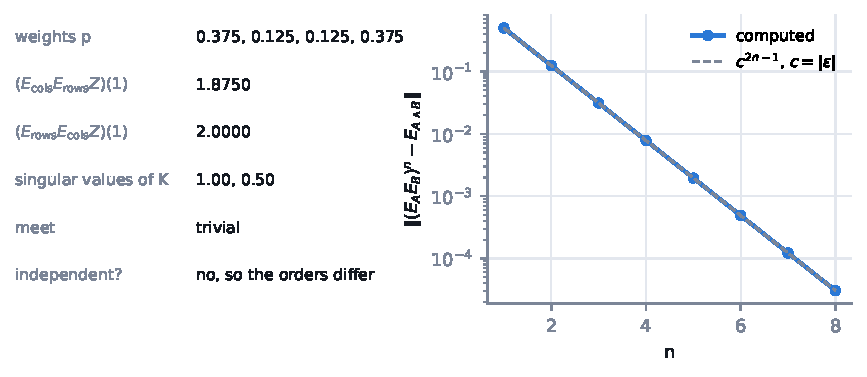
\includegraphics[width=\linewidth]{fig_algebra.pdf}
\caption{Algebra (\cref{thm:commute,thm:rate}). Four points with weights $\tfrac{1\pm\varepsilon}4$, pooled by rows and by columns, at
$\varepsilon=\tfrac12$ (\cref{ex:46}). The two orders give $1.875$ and $2.000$ at point $1$. The computed norms
$\lVert(E_AE_B)^n-E_{A\wedge B}\rVert$ lie on $c^{2n-1}$ with $c=\tfrac12$, from $0.5$ at $n=1$ to $3.05\times10^{-5}$ at $n=8$.}
\label{fig:algebra}
\end{figure}

\begin{figure}[!htbp]\centering
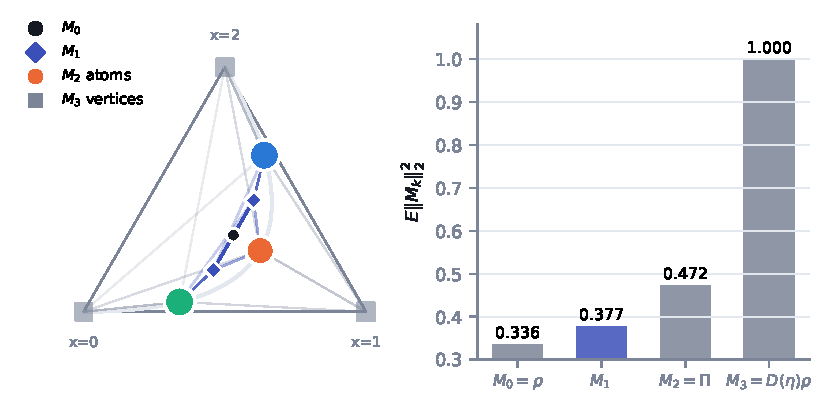
\includegraphics[width=0.92\linewidth]{fig_tower.pdf}
\caption{The tower as a martingale (\cref{prop:fibre,thm:martingale}). $M_0=\rho$ (black), the level-two barycentres $M_1$
(diamonds), the atoms $M_2$ of $\Pi$ (coloured, sized by mass) and the vertices $M_3$ (sized by $\rho$). Each position is a conditional
expectation of the next. The energies $E\lVert M_k\rVert_2^2=0.336,\ 0.377,\ 0.472,\ 1.000$ increase along the convex-order chain. The
outer pair, $\delta_\rho=\ebot\Pi$ and $\D(\eta)\rho=\etop\Pi$, are the two sides of the shift law's unit defect
(\cref{prop:beck-located}).}
\label{fig:tower}
\end{figure}

\begin{figure}[!htbp]\centering
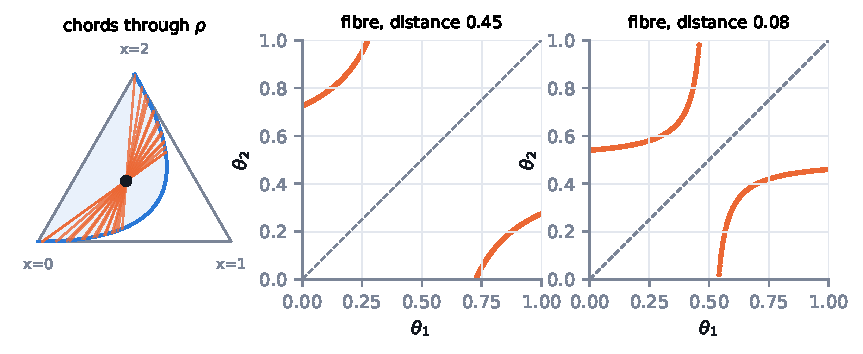
\includegraphics[width=\linewidth]{fig_secant.pdf}
\caption{Secant geometry (\cref{sec:secant}). Two-component mixtures of the curve fill its convex hull. The fibre over $\rho$ is the
family of chords through $\rho$, drawn as a curve in $(\theta_1,\theta_2)$ coordinates. It has two branches, exchanged by relabelling
the components. As $\rho$ approaches the curve (distance $0.45\to0.08$), the branches close in on the diagonal $\theta_1=\theta_2$, the
collision locus where the fibre becomes the weight-split segment (\cref{prop:walls}(b)).}
\label{fig:secant}
\end{figure}

\begin{figure}[!htbp]\centering
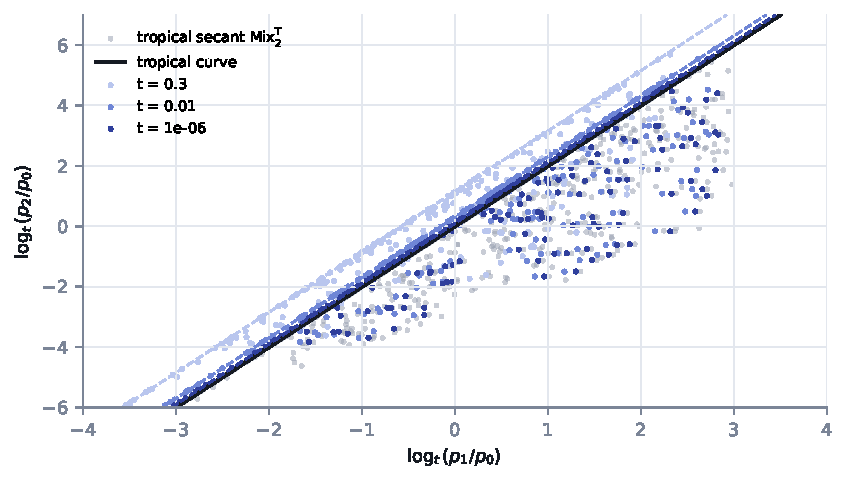
\includegraphics[width=0.86\linewidth]{fig_tropical.pdf}
\caption{The Berkovich retraction in the chart $(\log_t(p_1/p_0),\log_t(p_2/p_0))$ (\cref{thm:monad,thm:secant,thm:berk}). Grey: the
tropical secant $\min(w_1+u_1,w_2+u_2)$. Black: the tropical curve, which is the row space of the design. Coloured: the same 260
two-component mixtures at scales $t=0.3$, $10^{-2}$, $10^{-6}$, and the image of the curve (dashed, shifted by $\log_t2$). The largest
coordinate deviation from the tropical limit is $1.60$, $0.45$ and $0.13$. It decays like $1/\log(1/t)$, because only the
leading-coefficient corrections $\log_tc$ remain.}
\label{fig:tropical}
\end{figure}

\begin{figure}[!htbp]\centering
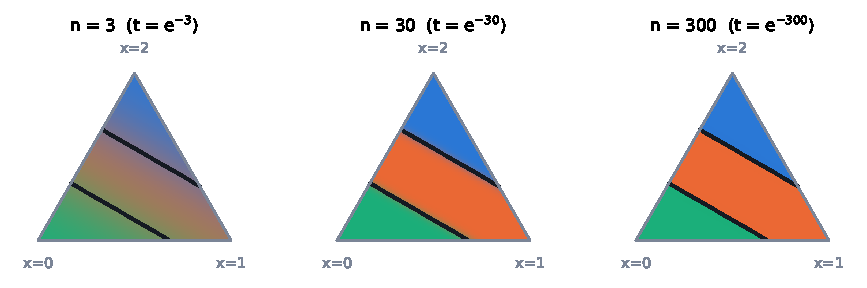
\includegraphics[width=\linewidth]{fig_walls.pdf}
\caption{Zero-temperature shadows (\cref{prop:posterior,prop:walls}). Each empirical distribution $q$ of $n$ observations is coloured
by the posterior over the three atoms, $\propto\Pi_i\exp(n\sum_xq(x)\log r_i(x))$. As $n$ grows, which is $t=e^{-n}\to0$, the colours
harden into cells. The black walls are the $n\to\infty$ tie loci; they are straight because log-likelihoods are linear in $q$. The
limiting map is nearest-atom pooling, discontinuous exactly on the walls (\cref{prop:continuity}).}
\label{fig:walls}
\end{figure}

\FloatBarrier

%=====================================================================
\section{Cohomology I: the $L^2$ presheaf and its Beck--Chevalley condition}\label{sec:presheaf}
%=====================================================================
Conditional expectations are the restriction maps of a presheaf, and the commutation theorem is its Beck--Chevalley condition. This
section makes both statements precise and measures the failure.

\begin{definition}[The $L^2$ presheaf]
Let $(\Omega,\mathcal F,\PP)$ be a probability space, and let $\mathcal S$ be the poset of sub-$\sigma$-algebras of $\mathcal F$
(completed), ordered by inclusion. The presheaf $\mathcal H$ on $\mathcal S$ is defined by
\[
\mathcal H(G)=L^2(G),\qquad \rho_{G'G}=E_G|_{L^2(G')}\colon\mathcal H(G')\to\mathcal H(G)\quad(G\subseteq G').
\]
Each restriction has a section, the inclusion $\iota_{GG'}\colon L^2(G)\hookrightarrow L^2(G')$, with $\rho_{G'G}\iota_{GG'}=\id$.
\end{definition}

\begin{lemma}
$\mathcal H$ is a presheaf: $\rho_{GG}=\id$ and $\rho_{G'G}\rho_{G''G'}=\rho_{G''G}$ for $G\subseteq G'\subseteq G''$.
\end{lemma}
\begin{proof}
This is the tower property $E_GE_{G'}=E_G$.
\end{proof}

\begin{definition}[Beck--Chevalley]
A commuting square of inclusions $C\subseteq A$, $C\subseteq B$, $A\subseteq D$, $B\subseteq D$ satisfies the \emph{Beck--Chevalley
condition} for $\mathcal H$ if
\[
\rho_{DA}\circ\iota_{BD}=\iota_{CA}\circ\rho_{BC}\colon L^2(B)\to L^2(A),
\]
that is, $E_Af=E_Cf$ for every $f\in L^2(B)$. Its \emph{defect} is the operator
$\beta_{A,B}=(\rho_{DA}\iota_{BD}-\iota_{CA}\rho_{BC})$ on $L^2(B)$.
\end{definition}

\begin{theorem}[Beck--Chevalley is conditional independence]\label{thm:bc}
Let $A,B$ be sub-$\sigma$-algebras (completed), $C=A\wedge B=A\cap B$, and $D\supseteq A\vee B$. The following are equivalent:
\begin{enumerate}[label=(\roman*)]
\item the Beck--Chevalley condition holds for the square $C\subseteq A,B\subseteq D$;
\item $E_AE_B=E_{A\wedge B}$ (condition (ii) of \cref{thm:commute});
\item $E_AE_B=E_BE_A$;
\item $A$ and $B$ are conditionally independent given $A\wedge B$.
\end{enumerate}
In general the defect satisfies
\[
\lVert\beta_{A,B}\rVert=\lVert E_AE_B-E_{A\wedge B}\rVert=c,
\]
where $c$ is the cosine of the Friedrichs angle between $L^2(A)$ and $L^2(B)$. For finite partitions, $c$ is the largest singular value
below $1$ of the normalised contingency matrix $K$. The condition is symmetric in $A$ and $B$.
\end{theorem}

\begin{proof}
Write $M=L^2(A)\cap L^2(B)$.

\emph{Step 0: $M=L^2(C)$.} The inclusion $\supseteq$ is clear. Conversely, let $f$ have an $A$-measurable version $f_A$ and a
$B$-measurable version $f_B$. For rational $q$, the sets $\{f_A>q\}\in A$ and $\{f_B>q\}\in B$ differ by a null set. Both
$\sigma$-algebras are complete, so each set lies in both, and $f_A$ is $A\cap B$-measurable.

\emph{Step 1: (i)$\Leftrightarrow$(ii).} By definition, (i) says $E_Ag=E_Cg$ for all $g\in L^2(B)$, that is, $E_AE_B=E_CE_B$. Since
$C\subseteq B$, the tower property gives $E_CE_B=E_C$.

\emph{Step 2: (ii)$\Rightarrow$(iii).} $E_C$ is self-adjoint, so $E_BE_A=(E_AE_B)^\ast=E_C^\ast=E_C=E_AE_B$.

\emph{Step 3: (iii)$\Rightarrow$(ii).} Put $P=E_AE_B$. Commutation gives $P^2=E_A^2E_B^2=P$ and $P^\ast=E_BE_A=P$, so $P$ is an
orthogonal projection. Its range lies in $L^2(A)$, and since $P=E_BE_A$ it also lies in $L^2(B)$, hence in $M$. Every $f\in M$ has
$Pf=f$. So $P$ is the projection onto $M=L^2(C)$, which is $E_C$.

\emph{Step 4: (ii)$\Rightarrow$(iv).} Let $U\in L^\infty(A)$, $V\in L^\infty(B)$ and $W\in L^\infty(C)$. Because $UW\in L^2(A)$ and
$E_AV=E_AE_BV=E_CV$,
\[
\EE[UVW]=\langle UW,E_AV\rangle=\langle UW,E_CV\rangle=\EE[U\,W\,E_CV]=\EE[E_CU\cdot E_CV\cdot W],
\]
where the last step conditions on $C$, using that $W\,E_CV$ is $C$-measurable. Hence $\EE[UV\mid C]=E_CU\cdot E_CV$.

\emph{Step 5: (iv)$\Rightarrow$(ii).} For bounded $U\in L^2(A)$ and $V\in L^2(B)$,
$\langle U,E_AV\rangle=\EE[UV]=\EE[E_CU\,E_CV]=\langle U,E_CV\rangle$. Bounded functions are dense in $L^2(A)$, so $E_AV=E_CV$. Both
sides are continuous in $V$ and bounded $V$ are dense in $L^2(B)$, so $E_AE_B=E_CE_B=E_C$.

\emph{Step 6: the norm.} Split $g\in L^2(B)$ as $g=g_M+g_\perp$ with $g_M\in M$ and $g_\perp\in L^2(B)\ominus M$. Then $\beta g_M=g_M-g_M=0$
and $E_Cg_\perp=0$, so $\beta g=E_Ag_\perp$. Moreover $E_Ag_\perp\perp M$, since $\langle E_Ag_\perp,m\rangle=\langle g_\perp,m\rangle=0$ for $m\in M$.
Hence
\[
\lVert\beta\rVert=\sup\big\{|\langle f,g\rangle|:\ f\in L^2(A)\ominus M,\ g\in L^2(B)\ominus M,\ \lVert f\rVert=\lVert g\rVert=1\big\},
\]
which is the definition of the Friedrichs cosine \cite{Deutsch2001}. Also $E_AE_B-E_C=(E_A-E_C)E_B=\beta E_B$, and $E_B$ maps the unit ball
of $L^2(D)$ onto that of $L^2(B)$, so $\lVert E_AE_B-E_C\rVert=\lVert\beta\rVert$.

\emph{Step 7: the finite formula.} In the bases $1_a/\sqrt{p(a)}$ and $1_b/\sqrt{p(b)}$, $E_A|_{L^2(B)}$ has matrix $K$. Its singular values
are the cosines of the principal angles, and the value $1$ belongs exactly to $M$ (\cref{lem:meet}). Removing $M$ leaves the largest
remaining singular value. Symmetry follows from (iv).
\end{proof}

\begin{remark}[Reading the theorem]
The lattice of $\sigma$-algebras, or of partitions, which are assignments of outcomes to cells, carries the presheaf
$\sigma\mapsto L^2(\sigma)$. Its restriction maps are conditional expectations. Two restrictions interchange exactly when the square
through the meet is Beck--Chevalley, and the size of the failure is one number, the Friedrichs cosine. The same number is the exact rate
of alternating projections (\cref{thm:rate}), so it measures both how far the square is from commuting and how fast iterated
restriction forgets the difference.
\end{remark}

Check H1 verifies the equivalence on 300 random squares (199 conditionally independent, 101 not), and H2 verifies
$\lVert\beta\rVert=c$.

\subsection{Gluing and the degree-one obstruction}
For a cover $\{A,B\}$ of $D$ with overlap $C=A\wedge B$, form the Čech-type complex
\[
0\to L^2(D)\xrightarrow{\ \delta^0\ }L^2(A)\oplus L^2(B)\xrightarrow{\ \delta^1\ }L^2(C)\to0,
\]
with $\delta^0f=(E_Af,E_Bf)$ and $\delta^1(f_A,f_B)=E_Cf_A-E_Cf_B$.
A pair in $\ker\delta^1$ is \emph{compatible}: it agrees on the overlap. A \emph{gluing} of a compatible pair is an $f$ with
$\delta^0f=(f_A,f_B)$. The degree-one cohomology is $\check H^1=\ker\delta^1/\operatorname{im}\delta^0$.

\begin{theorem}[Gluing]\label{thm:gluing}
\begin{enumerate}[label=(\alph*)]
\item $\delta^1\delta^0=0$, and $\delta^1$ is surjective.
\item $\overline{\operatorname{im}\delta^0}=\ker\delta^1$. Hence $\check H^1=0$ iff $\operatorname{im}\delta^0$ is closed, iff
  $L^2(A)+L^2(B)$ is closed, iff $c<1$. This always holds in finite dimensions, so every compatible pair glues.
\item If $c=1$, then $\check H^1$ is nonzero and non-Hausdorff: its reduced version $\ker\delta^1/\overline{\operatorname{im}\delta^0}$
  vanishes, but some compatible pairs do not glue.
\item Under Beck--Chevalley the gluing is canonical: $f=f_A+f_B-E_Cf_A$. This formula glues every compatible pair iff
  Beck--Chevalley holds.
\item Gluings are not unique: $\ker\delta^0=L^2(D)\ominus\big(L^2(A)+L^2(B)\big)$, which is nonzero unless
  $L^2(D)=\overline{L^2(A)+L^2(B)}$. So $\mathcal H$ satisfies the existence half of the sheaf condition (when $c<1$), but not the
  uniqueness half.
\end{enumerate}
\end{theorem}
\begin{proof}
(a) $E_CE_A=E_C=E_CE_B$, and $\delta^1(f,0)=E_Cf$ is onto $L^2(C)$.
(b) The adjoint is $(\delta^0)^*(u,v)=u+v$, with kernel $\{(u,-u):u\in L^2(A)\cap L^2(B)=L^2(C)\}$. So
$\overline{\operatorname{im}\delta^0}=\{(f_A,f_B):f_A-f_B\perp L^2(C)\}=\ker\delta^1$. By the closed range theorem,
$\operatorname{im}\delta^0$ is closed iff $\operatorname{im}(\delta^0)^*=L^2(A)+L^2(B)$ is closed, which holds iff $c<1$
\cite{Deutsch2001}.
(c) A dense, non-closed range is a proper subspace of its closure.
(d) If Beck--Chevalley holds, $E_Af=f_A+E_Cf_B-E_Cf_A=f_A$, and symmetrically for $B$. Conversely, the pair $(f_A,E_Cf_A)$ is
compatible, and the formula returns $f=f_A$, which glues it iff $E_Bf_A=E_Cf_A$. Requiring this for all $f_A$ is Beck--Chevalley.
(e) $\ker\delta^0=L^2(A)^\perp\cap L^2(B)^\perp$.
\end{proof}

Checks H3 and H4 verify (b) and (d) exactly on 300 squares.

\begin{proposition}[Comparisons are restrictions, not gluing isomorphisms]\label{prop:not-iso}
Each Beck comparison computed in this paper (\cref{prop:single-step}) is a restriction $\rho_{G'G}$ with $G\subsetneq G'$. Such a map is
surjective and not injective, and it strictly lowers the norm off $L^2(G)$. In particular no comparison map is an isomorphism, so the
comparisons cannot be the gluing isomorphisms of a structure sheaf. What they are is the structure maps of $\mathcal H$. The
interchange of two of them is the Beck--Chevalley condition (\cref{thm:bc}), and its failure is measured by $c$.
\end{proposition}
\begin{proof}
$\rho_{G'G}\iota_{GG'}=\id$ gives surjectivity, and $L^2(G')\ominus L^2(G)\ne0$ is its kernel. Pythagoras gives the strict decrease (check
H5).
\end{proof}

\FloatBarrier
%=====================================================================
\section{Cohomology II: fibres as topology}\label{sec:fibre-topology}
%=====================================================================
Classical barycentre fibres are convex (\cref{prop:fibre}), so their topology is trivial. So are the tower's level-two lifting fibres,
which are polytopes \cite[Def.~10.14]{Tower}. Nontrivial topology appears in two places: when components are constrained to a curved
model, and in tropical fibres, which are unions of polyhedra. This section computes the second kind exactly.

\subsection{The cover by assignment cells}
For the Hardy--Weinberg model, a tropical two-component decomposition has parameters $\vartheta=(\beta,d_1,d_2)\in\R^3$. Here $\beta$ is
the weight difference, $w_1=\max(0,-\beta)$, $w_2=\max(0,\beta)$, and $d_i$ is the rate of component $i$, so that by \cref{thm:secant}
$u(d)=(0,d,2d)-\min(0,2d)$. The \emph{tropical fibre} over a target $v\in\DT X$ is
\[
F_v=\big\{\vartheta:\ \min_i\big(w_i+u(d_i)(x)\big)=v(x)\ \text{for all }x\big\}.
\]

\begin{definition}[Assignment cells]
For $\alpha\colon X\to\{1,2\}$ (a designated attainer for each outcome) and a sign pattern $\sigma\in\{\pm\}^3$ of $(\beta,d_1,d_2)$, let
\[
P_{\alpha,\sigma}=\big\{\vartheta\in\text{orthant }\sigma:\ w_{\alpha(x)}+u(d_{\alpha(x)})(x)=v(x),\ \ w_j+u(d_j)(x)\ge v(x)\ \forall j,x\big\}.
\]
\end{definition}

\begin{lemma}
Each $P_{\alpha,\sigma}$ is a closed convex polyhedron. The cells cover $F_v$, and every intersection of cells is a polyhedron.
\end{lemma}
\begin{proof}
Within an orthant every term is affine in $\vartheta$, so each cell is defined by finitely many affine equalities and inequalities. A
point of $F_v$ lies in the cell given by its orthant and by any choice of attainer at each $x$.
\end{proof}

\begin{theorem}[Fibre cohomology from the nerve]\label{thm:nerve}
Let $N_v$ be the nerve of the cover $\{P_{\alpha,\sigma}\}$. Then $H^\ast(F_v;\mathbb Q)\cong\check H^\ast(\{P_{\alpha,\sigma}\};\mathbb Q)\cong
H^\ast(N_v;\mathbb Q)$. A set of cells spans a face of $N_v$ iff its joint system of affine constraints is feasible. By Farkas' lemma,
it is \emph{not} a face iff there is a certificate $(y_{\mathrm{eq}},y_{\mathrm{ub}}\ge0)$ with
$A_{\mathrm{eq}}^\top y_{\mathrm{eq}}+A_{\mathrm{ub}}^\top y_{\mathrm{ub}}=0$ and $b_{\mathrm{eq}}\cdot y_{\mathrm{eq}}+b_{\mathrm{ub}}\cdot y_{\mathrm{ub}}<0$.
So the cohomology of the fibre is determined by which assignment patterns are certified impossible.
\end{theorem}
\begin{proof}
The nerve theorem holds for finite covers by closed convex sets in $\R^d$: every nonempty intersection is convex, hence
contractible \cite{Bjorner1995}. The face criterion is Farkas' lemma \cite{Schrijver1986}.
\end{proof}

These certificates have the same form as the tower's lifting certificates \cite[Thm.~10.8, Thm.~10.13(iii)]{Tower}. There, a
separating functional certifies that a claim has no admissible lift. Here, a Farkas vector certifies that a pattern of attainers has no
tropical decomposition. \Cref{thm:nerve} upgrades such certificates from yes/no answers to cohomological data: the complex of
patterns that are \emph{not} certified impossible computes the homology of the fibre.

\subsection{Local lifts as sections}
\begin{proposition}[Local lifts]\label{prop:local-lifts}
Work in the full simplex model $\DK X$, and fix a positive $\rho$ with $\val\rho=v$.
\begin{enumerate}[label=(\alph*)]
\item For each cell, the construction in the proof of \cref{thm:lift}, with the remainder at $x$ given to $\alpha(x)$, is a section of
  $\val$ over the rational points of the cell.
\item Over a fixed tropical point, the set of lifts is convex. A convex combination of two exact decompositions of $\rho$ with the same
  valuation pattern is again one, because leading coefficients of positive terms add without cancelling.
\item Consequently, on every nonempty face of the nerve, local lifts from different cells are joined by a segment of lifts. The
  lifting data add no obstruction beyond the emptiness certificates of \cref{thm:nerve}.
\end{enumerate}
\end{proposition}
\begin{proof}
(a) is \cref{thm:lift} with designated attainers. (b) holds because the decomposition equations are linear in $(q_i(x))$, and the
valuation pattern is fixed by positivity (check K4). (c) follows from (b) on each common point.
\end{proof}

For a model $V$, lifting into $V$ is \cref{op:ident}. A lifting failure inside $V$ would be a new kind of certificate. Its interaction
with the nerve is the natural next computation.

\subsection{The computation for Hardy--Weinberg}
\begin{figure}[!htbp]\centering
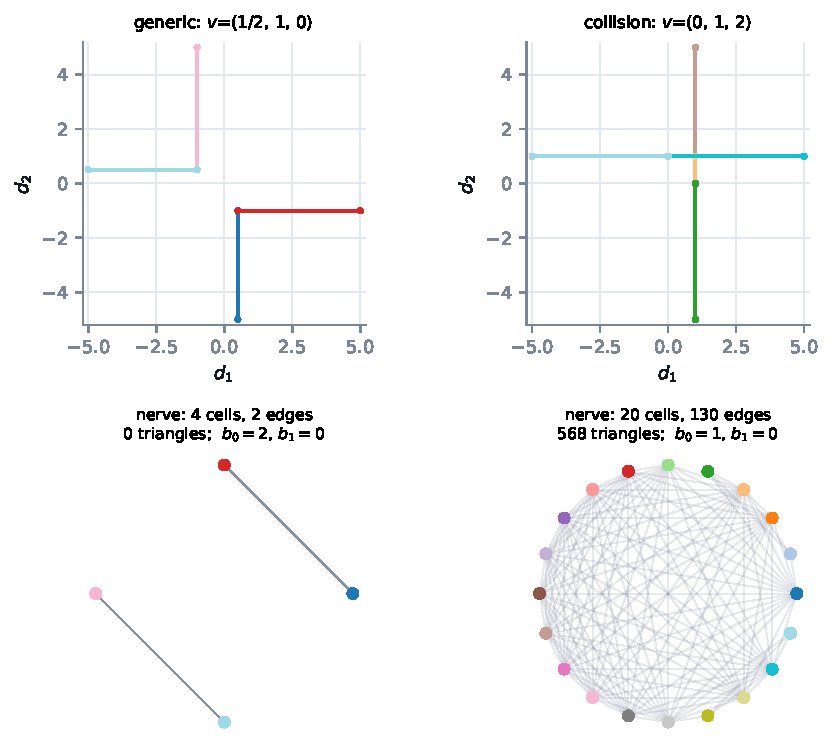
\includegraphics[width=0.92\linewidth]{fig_fibres.pdf}
\caption{Tropical fibres $F_v$ projected to $(d_1,d_2)$, coloured by assignment cell, and their nerves.
\emph{Generic} $v=(\tfrac12,1,0)$: four cells and two edges. There are two components, each a bent line, exchanged by swapping the
components, and $b_0=2$, $b_1=0$. \emph{Collision} $v=(0,1,2)$, on the tropical curve: twenty cells, $130$ edges and $568$ triangles.
The branches are joined, and $b_0=1$, $b_1=0$.}
\label{fig:fibres}
\end{figure}

\begin{theorem}[Topology of the Hardy--Weinberg fibres]\label{thm:hw-topology}
For the generic target $v=(\tfrac12,1,0)$, $F_v$ has Betti numbers $(b_0,b_1)=(2,0)$. Its two components are exchanged by the label swap
$(\beta,d_1,d_2)\mapsto(-\beta,d_2,d_1)$. For the collision target $v=(0,1,2)$, which lies on the tropical curve, $(b_0,b_1)=(1,0)$.
\end{theorem}
\begin{proof}
Exact computation (checks K1--K3). Every nonempty cell and face has an exact rational witness: 6 for the generic target and 718 for
the collision target. Every empty cell and face among the candidates has an exact Farkas certificate: 64 and 104 respectively. The
Betti numbers are ranks over $\mathbb Q$ of the coboundary matrices of the nerve.
\end{proof}

\begin{figure}[!htbp]\centering
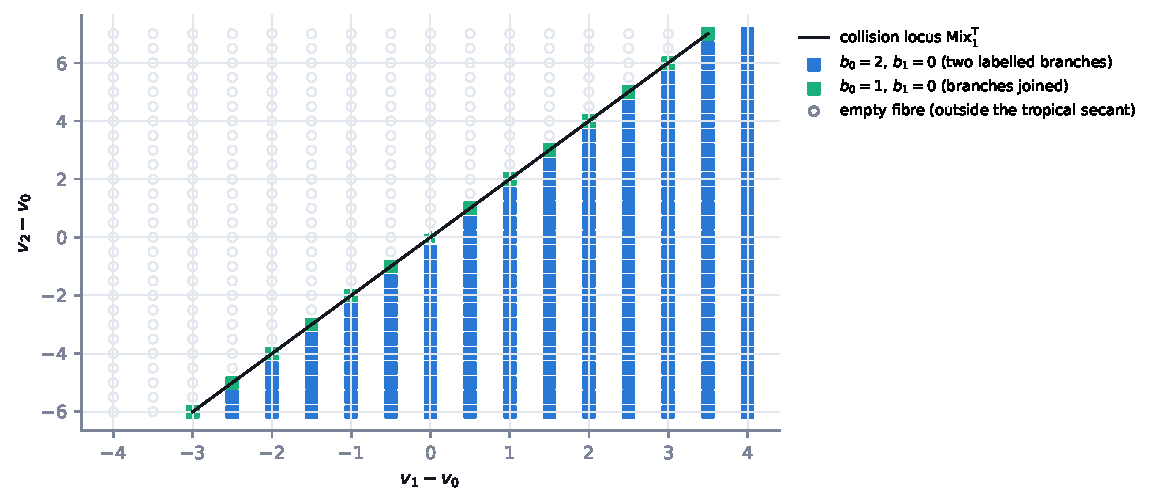
\includegraphics[width=0.95\linewidth]{fig_betti.pdf}
\caption{The homology of the fibre as a function of the target, over a grid of $17\times27$ targets in the chart
$(v_1-v_0,v_2-v_0)$. Of these, 236 lie outside the tropical secant (empty fibre). On the 209 targets inside the secant and off the collision locus,
$b_0=2$; on the 14 targets on the locus, $b_0=1$. $b_1=0$ wherever it was computed, which is every target except $v=(0,0,0)$, where
all 64 cells are nonempty and only $b_0$ was computed. This is the homological form of the collision wall of \cref{sec:secant}.}
\label{fig:betti}
\end{figure}

\paragraph{Reading.} Over a generic target there are two continuous families of decompositions, one for each labelling. On the
collision locus a component may coincide with the other, and the families merge. The same jump appears classically in
\cref{fig:secant}, where the two branches of the classical fibre meet the diagonal. Homology turns the proposed wall-crossing of
\cref{conj:wall} into a computable invariant. In this example the jump is $\Delta b_0=-1$ across the collision locus, with no change in
$b_1$. On the scanned grid, tie walls in the target (\cref{prop:walls}(a)) change the cell structure of the fibre but not its homology.

\FloatBarrier
%=====================================================================
\section{Example: hallucination in a three-token model}\label{sec:halluc}
%=====================================================================
This section connects the $L^2$ presheaf to the tower's notion of hallucination \cite[\S10.5]{Tower}. A hallucination there is an
\emph{obstructed claim}: a statement that is admissible locally but has no coherent completion. We use the smallest model in which this
happens, three token positions observed pairwise. Every number below is checked exactly by \texttt{check\_hallucination.py}.

\subsection{The model}
Three binary token positions $X_0,X_1,X_2$ are seen through the contexts (windows) $\{0,1\}$, $\{1,2\}$ and $\{0,2\}$. In each context
the two tokens agree with probability $\varepsilon$:
\[
P_{X_iX_j}=\begin{pmatrix}\varepsilon/2&(1-\varepsilon)/2\\(1-\varepsilon)/2&\varepsilon/2\end{pmatrix}.
\]
The tables come from a mixture of sources $s\in\{A,B,U\}$, each with its own agreement $\varepsilon_s$. With weights $w$ in the simplex,
the pairwise tables mix linearly:
\[
\varepsilon(w)=w_A\varepsilon_A+w_B\varepsilon_B+w_U\varepsilon_U .
\]
We take $\varepsilon_A=0.20$, $\varepsilon_B=0.30$ and $\varepsilon_U=0.40$.

\subsection{Hallucination is a failure of gluing}
\begin{proposition}[Global sections and their certificate]\label{prop:three-bit}
\begin{enumerate}[label=(\alph*)]
\item A joint law of $(X_0,X_1,X_2)$ with these pairwise tables exists iff $\varepsilon\ge\tfrac13$.
\item For $\varepsilon<\tfrac13$, the functional $\Phi(P)=\sum_{i<j}P(X_i\ne X_j)$ certifies the obstruction. Every joint has $\Phi\le2$,
  because each of the eight joint outcomes has at most two disagreeing pairs. The pairwise tables give $\Phi=3(1-\varepsilon)$,
  which exceeds $2$ by exactly $1-3\varepsilon$.
\item For $\varepsilon\ge\tfrac13$, the global sections form the segment $J+s\chi$, $|s|\le\min(a,b)$. Here
  $\chi(x)=(-1)^{x_0+x_1+x_2}$ spans the one-dimensional kernel of the pairwise-margin map, and $J$ is the symmetric joint with
  $a=\tfrac{3\varepsilon-1}4$ on $000$ and $111$ and $b=\tfrac{1-\varepsilon}4$ on the other six outcomes.
\end{enumerate}
\end{proposition}
\begin{proof}
(a) and (b): this is \cite[Thm.~4.8]{Conditionals} at $\tau=0$. All three correlations are $E_{ij}=2\varepsilon-1$, and the
3-cycle inequality with all signs negative reads $-3(2\varepsilon-1)\le1$. The bound $\Phi\le2$ is checked atom by atom. (c) The margin
map has rank $7$ on $\R^8$, and $\chi$ lies in its kernel. $J$ reproduces the tables. Nonnegativity of $J+s\chi$ gives the range of
$s$ (checks L1, L2).
\end{proof}

In the language of \cite[\S10]{Tower}, each pairwise table is an admissible local claim, and for $\varepsilon<\tfrac13$ the family is an
obstructed claim. Its certificate is the test function $\Phi$, a separating functional of the kind in \cite[Thm.~10.8]{Tower}. The
parity $\chi$ is not a certificate. It indexes the non-uniqueness of the joint when one exists.

\subsection{The wall in weight space, and a token stream}
By \cref{prop:three-bit}, the mixture is liftable iff $\varepsilon(w)\ge\tfrac13$. This is a half-space in the weight simplex: the wall
$\varepsilon(w)=\tfrac13$ is a straight line, and the liftable side is the side of the coherent source $U$ (the only source with
$\varepsilon_s\ge\tfrac13$). In the coordinates $\theta=w_A/(w_A+w_B)$ and $\mu=w_U$, the wall becomes the curve
$\mu(\theta)=(\tfrac13+\theta)/(1+\theta)$. The liftable side is $\mu\ge\mu(\theta)$: more weight on the coherent source restores a joint.

For the 12-step stream $(\theta_t,\mu_t)=(0.10,0.10),(0.20,0.15),\dots,(0.30,0.90)$ of \cref{fig:hallucination}, the agreement
$\varepsilon_t$ rises from $0.301$ to $0.387$. The stream is obstructed (hallucinating) for $t=1,\dots,7$, with $\varepsilon_7=0.332$, and
liftable from $t=8$, with $\varepsilon_8=0.337$. The transition is the crossing of the wall between steps $7$ and $8$ (check L6). This
wall is classical: it is linear in the weights, and it is not a tropical wall (\cref{sec:halluc-trop}).

\begin{figure}[!htbp]\centering
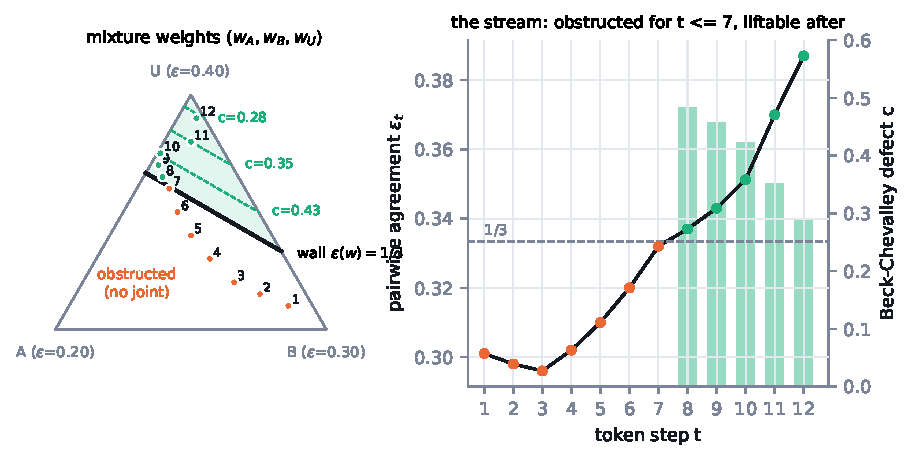
\includegraphics[width=\linewidth]{fig_hallucination.pdf}
\caption{The three-token hallucination example. Left: the weight simplex. The straight wall $\varepsilon(w)=\tfrac13$ separates the
obstructed region (no joint law) from the liftable region (shaded). Dashed lines are level sets of the Beck--Chevalley defect $c$ of the
symmetric joint, and points are the 12 stream steps (orange obstructed, green liftable). Right: $\varepsilon_t$ along the stream, which
crosses $\tfrac13$ between $t=7$ and $t=8$, and the defect $c_t$ (bars) once a joint exists.}
\label{fig:hallucination}
\end{figure}

\subsection{The $L^2$ presheaf on context windows}
Once the claim is liftable, choose a full-support global section $P$ (for instance $J$, for $\tfrac13<\varepsilon<1$). This gives a
probability space, and the windows give two $\sigma$-algebras on it:
\[
A=\sigma(X_0,X_1),\qquad B=\sigma(X_1,X_2).
\]
Their shadows $E_A$ and $E_B$ are what a reader confined to one window can compute.

\begin{proposition}[Window shadows]\label{prop:windows}
For a full-support section $P$:
\begin{enumerate}[label=(\alph*)]
\item the meet is $A\wedge B=\sigma(X_1)$, the shared token;
\item the window square satisfies Beck--Chevalley iff $X_0\perp X_2\mid X_1$ under $P$, that is, iff the sequence is Markov through the
  shared token;
\item the defect is $c=\max_{x_1}\big|\operatorname{corr}_P(X_0,X_2\mid X_1=x_1)\big|$, and alternating the two window shadows converges
  to $E[\,\cdot\mid X_1]$ at rate $c^{2n-1}$;
\item at the symmetric section $J$, $c=\dfrac{|2\varepsilon-1|}{2\varepsilon}$;
\item a Markov section exists in the segment $J+s\chi$ iff $\varepsilon=\tfrac12$ (for $\tfrac13<\varepsilon<1$). On 99 sections across
  the segment, the defect is smallest at the symmetric section.
\end{enumerate}
\end{proposition}
\begin{proof}
(a) The cells of $A$ are values of $(x_0,x_1)$ and those of $B$ values of $(x_1,x_2)$. Two cells meet iff they share $x_1$, so the
components of $G(A,B)$ are the two values of $x_1$ (\cref{lem:meet}).
(b) This is \cref{thm:bc}(iv) with meet $\sigma(X_1)$.
(c) $K$ is block diagonal over the two components. Each block is the normalised $2\times2$ table of $(X_0,X_2)$ given $X_1=x_1$, whose
singular values are $1$ and the absolute correlation. Now apply \cref{thm:bc,thm:rate}.
(d) Given $X_1=0$, the table of $(X_0,X_2)$ is proportional to $\begin{psmallmatrix}a&b\\b&b\end{psmallmatrix}$. Its correlation is
$(a-b)/(2(a+b))=(2\varepsilon-1)/(2\varepsilon)$, and the case $X_1=1$ is symmetric.
(e) Under the Markov property, $P(X_0=X_2\mid X_1)=\varepsilon^2+(1-\varepsilon)^2$. This must equal the table value $\varepsilon$, so
$\varepsilon\in\{\tfrac12,1\}$. The minimisation is computed (checks L3--L5, L7).
\end{proof}

\paragraph{Reading.} Two context windows that share a token commute as conditional expectations exactly when everything the first
token says about the third passes through the shared token. The defect $c$ is the long-range coupling that no single window
represents, and $c^{2n-1}$ is how fast repeated window-by-window conditioning forgets it. Along the stream, once a joint exists the
defect falls from $c_8=0.484$ to $c_{12}=0.292$ as weight moves to the coherent source. It never reaches $0$, because $\varepsilon=\tfrac12$
is not attainable with these sources.

\subsection{Three layers of obstruction}
\begin{center}\small
\begin{tabular}{>{\raggedright}p{2.6cm}>{\raggedright}p{4.6cm}>{\raggedright\arraybackslash}p{6.6cm}}\toprule
regime & structure & certificate or measure\\\midrule
$\varepsilon<\tfrac13$ & no global section (hallucination) & $\Phi>2$, by $1-3\varepsilon$ (\cref{prop:three-bit})\\
$\tfrac13\le\varepsilon<1$, $\varepsilon\ne\tfrac12$ & sections form a segment; windows do not commute & Beck--Chevalley defect $c>0$ (\cref{prop:windows})\\
$\varepsilon=\tfrac12$ & a Markov section exists & $c=0$ at that section\\
\bottomrule
\end{tabular}
\end{center}
The first layer is a failure of gluing for the presheaf of distributions on the context cover. The second is the Beck--Chevalley defect
of the $L^2$ presheaf on the glued space. The tower's obstructed claims live in the first layer. The $L^2$ presheaf measures what
remains once the claim is coherent.

The two layers are logically independent: a gluing failure does not imply a Beck--Chevalley defect, nor the reverse. The next
proposition makes this exact. Gluing failure comes from cycles in the cover; the defect comes from coupling inside the glued space.

\begin{proposition}[Two windows always glue; failure needs a cycle]\label{prop:two-layers}
\begin{enumerate}[label=(\alph*)]
\item Let $U,V,W$ be finite random variables, and let $P_{UV}$ and $P_{VW}$ be full-support laws with the same $V$-marginal $P_V$. Then
  \[
  P(u,v,w)=\frac{P_{UV}(u,v)\,P_{VW}(v,w)}{P_V(v)}
  \]
  is a joint law with these two windows. It is the only one in which $U\perp W\mid V$, that is, the only one for which the windows
  $\sigma(U,V)$ and $\sigma(V,W)$ satisfy Beck--Chevalley. Every other gluing violates $U\perp W\mid V$. So a cover by two windows never fails
  to glue.
\item More generally, every compatible family of marginals on a cover glues whenever the cover is acyclic, that is, its windows can
  be removed one at a time so that each removed window meets the rest inside a single remaining window \cite{Vorobev1962}. The three
  pair windows of \cref{prop:three-bit} are not acyclic: their nerve is a hollow triangle ($b_1=1$; check M8), and
  \cref{prop:three-bit} exhibits the failure for $\varepsilon<\tfrac13$.
\item The defect does not detect the failure. As $\varepsilon\downarrow\tfrac13$ the fibre shrinks to the single section $J$, where
  $c=|2\varepsilon-1|/(2\varepsilon)=\tfrac12$. So at the wall the defect is bounded away from $1$, and a gluing failure is not a limit
  of large Beck--Chevalley defects. In the $L^2$ sense nothing fails at all: in finite dimensions $c<1$, so every compatible pair of
  $L^2$ sections glues (\cref{thm:gluing}(b)).
\end{enumerate}
\end{proposition}
\begin{proof}
(a) Summing over $w$ gives $P_{UV}$, and summing over $u$ gives $P_{VW}$, because both share $P_V$. The law factorises as
$P(u\mid v)P(w\mid v)P(v)$, so $U\perp W\mid V$. Conversely, conditional independence given $V$ forces
$P(u,w\mid v)=P(u\mid v)P(w\mid v)$, which with the two windows fixed determines $P$. Full support makes the meet
$\sigma(U,V)\wedge\sigma(V,W)$ equal to $\sigma(V)$, since every $u$ is joined to every $w$ through each $v$. Then \cref{thm:bc} identifies
Beck--Chevalley with $U\perp W\mid V$.
(b) Glue the windows in the removal order, applying (a) at each step with $V$ the overlap of the removed window with the rest; this is
Vorob'ev's theorem \cite{Vorobev1962}. For the three pair windows, removing any one leaves an overlap of two singletons
$\{X_i\},\{X_j\}$ that no single remaining window contains, so no removal order exists.
(c) At $\varepsilon=\tfrac13$, $a=0$, so $|s|\le\min(a,b)=0$ and the fibre is $\{J\}$. \Cref{prop:windows} gives
$c=|2\varepsilon-1|/(2\varepsilon)$ at $J$, which is $\tfrac12$ at $\varepsilon=\tfrac13$: given $X_1=0$ the table of $(X_0,X_2)$ is $\bigl(\begin{smallmatrix}0&b\\b&b\end{smallmatrix}\bigr)$, with correlation $-\tfrac12$, and likewise given $X_1=1$ (the formula is check L4b). In finite dimensions the Friedrichs
angle between $L^2(A)\ominus L^2(C)$ and $L^2(B)\ominus L^2(C)$ is positive, so $c<1$.
\end{proof}

\subsection{What tropicalisation sees}\label{sec:halluc-trop}
\begin{proposition}[Tropical shadow of hallucination]\label{prop:halluc-trop}
Over a real non-Archimedean field:
\begin{enumerate}[label=(\alph*)]
\item valuation commutes with marginalisation, so if the tropical tables have no tropical joint, the classical tables have no joint;
\item the hallucination at constant $\varepsilon<\tfrac13$ is invisible tropically: all entries have valuation $0$, and the zero tropical
  joint exists;
\item a scaled family with agreement $\varepsilon=\kappa t^{\alpha}$, $\alpha>0$, is tropically obstructed. The certificate is
  combinatorial: every outcome has an agreeing pair, so every tropical joint entry is at least $\alpha$, while the disagreement cells
  require $0$.
\end{enumerate}
\end{proposition}
\begin{proof}
(a) Marginalisation is pushforward, and \cref{thm:monad} gives $\val(\D f(P))=\D_{\T}f(\val P)$. (b) and (c) are direct (check L8).
\end{proof}

So the tropical shadow of a hallucination certificate is a support-level certificate: strong contextuality in the sense of
\cite{AbramskyBrandenburger2011}, graded by rates. It is sufficient but not necessary. The boundary $\varepsilon=\tfrac13$ concerns leading
coefficients, which the valuation discards. Hallucination is therefore \emph{not} in general a tropical wall crossing. The wall that
detects it is classical and linear in the weights (\cref{fig:hallucination}). The tropical walls of \cref{prop:walls} detect only
obstructions that are visible in rates.

\FloatBarrier
%=====================================================================
\section{Places: the context presheaf over $\mathcal{M}(\mathbb{Z})$}\label{sec:places}
%=====================================================================
The data of \cref{sec:halluc} are rational, so the context presheaf can be read at every place of $\mathbb{Q}$ at once. The setting
that holds all the places together is the Berkovich spectrum $\mathcal{M}(\mathbb{Z})$ \cite[Ex.~1.4.1]{Berkovich1990}, studied in
detail by Poineau \cite{Poineau2010}. This section shows that the places separate the gluing problem by the \emph{kind} of condition
involved, not by context. The contexts stay in the lattice; the places sort the linear, positive and valuative parts of the
problem. The sheaf-theoretic reading of contextuality is due to Abramsky and Brandenburger \cite{AbramskyBrandenburger2011}, and the
underlying marginal problem goes back to Vorob'ev \cite{Vorobev1962}. The new points here are the place-by-place decomposition and its
consequences for the Beck--Chevalley defect.

\paragraph{The space.} $\mathcal{M}(\mathbb{Z})$ is the set of multiplicative seminorms on $\mathbb{Z}$ bounded by the usual absolute value.
By Ostrowski's theorem it is a tree with one centre:
\begin{itemize}
\item the trivial seminorm $a_0$, whose residue field is $\mathbb{Q}$ with the trivial absolute value; by Poineau's description the
  germs of analytic functions at $a_0$ form the field $\mathbb{Q}$;
\item for each prime $p$ a branch $\{|\cdot|_p^{\alpha}:\alpha\in(0,\infty)\}$, whose points have completed residue field
  $\mathbb{Q}_p$, ending at the seminorm with kernel $p\mathbb{Z}$ and residue field $\mathbb{F}_p$;
\item one archimedean branch $\{|\cdot|_\infty^{\varepsilon}:\varepsilon\in(0,1]\}$.
\end{itemize}
Every neighbourhood of $a_0$ contains all but finitely many branches in full. A tree is contractible.

Throughout, $J+s\chi$ is the family of \cref{prop:three-bit}: $a=(3\varepsilon-1)/4$, $b=(1-\varepsilon)/4$, $J(000)=J(111)=a$,
$J=b$ elsewhere, and $\chi(x)=(-1)^{x_0+x_1+x_2}$.

\begin{proposition}[The centre: signed sections always exist]\label{prop:places-centre}
For every $\varepsilon\in\mathbb{Q}\cap(0,1)$ and every field $K\supseteq\mathbb{Q}$, the signed measures on $\{0,1\}^3$ over $K$ whose
three pair tables equal the window data form the line $\{J+s\chi:s\in K\}$. In particular the window data glue over $\mathbb{Q}$, and
over every $\mathbb{Q}_p$, for all $\varepsilon$, including $\varepsilon<\tfrac13$, where $a<0$.
\end{proposition}
\begin{proof}
$J$ has total mass $1$ and the right pair tables by direct computation. The pair-marginal map $K^8\to K^{12}$ has rank $7$: in the
character basis $\{(-1)^{\langle u,x\rangle}\}$ the pair tables determine every Fourier coefficient with $|u|\leq2$, and the only
character they do not see is $\chi$, the one with $u=(1,1,1)$. So the kernel is $K\chi$. Checks M1 and M2 verify both statements
exactly; M2 also finds rank $7$ over $\mathbb{F}_p$ for $p=2,3,5,7,11$.
\end{proof}

\begin{proposition}[Positivity is archimedean]\label{prop:places-order}
The positive fibre $\{s:J+s\chi\geq0\}$ is non-empty iff $\varepsilon\geq\tfrac13$. The order used here is the unique ordering of
$\mathbb{Q}$, which is the one induced by the archimedean place. No $\mathbb{Q}_p$ admits an ordering, because $-1$ is a sum of squares
in $\mathbb{Q}_p$. Hence the obstruction of \cref{prop:three-bit}, with its certificate $\Phi=\sum P(X_i\neq X_j)\leq2$, is supported at
the archimedean place: at $a_0$ and along every finite branch the data glue (\cref{prop:places-centre}).
\end{proposition}
\begin{proof}
The first statement is $\min(a,b)\geq0\iff\varepsilon\geq\tfrac13$. A field is orderable iff $-1$ is not a sum of squares (Artin--Schreier).
In $\mathbb{Q}_p$ every quadratic form in at least five variables is isotropic \cite[Ch.~IV, Thm.~6]{Serre1973}, so
$x_1^2+\dots+x_4^2+x_5^2$ has a non-trivial zero, and $-1$ is a sum of four squares. Check M3 confirms the first statement on a grid and
exhibits explicit witnesses for every $p\leq47$, lifted by Hensel's lemma to precision $p^{12}$ (for $p=2$ through $\sqrt{-7}\in\mathbb{Z}_2$).
\end{proof}

\begin{proposition}[Beck--Chevalley at the centre, its size at the places]\label{prop:places-bc}
For the windows $\sigma(X_0,X_1)$ and $\sigma(X_1,X_2)$, let $\Delta_{x_1}$ be the determinant of the $2\times2$ table of $(X_0,X_2)$
given $X_1=x_1$. On the family $J+s\chi$,
\[
\Delta_0=\tfrac18\bigl(4s-(2\varepsilon-1)(\varepsilon-1)\bigr),\qquad \Delta_1=-\tfrac18\bigl(4s+(2\varepsilon-1)(\varepsilon-1)\bigr).
\]
\begin{enumerate}[label=(\alph*)]
\item Beck--Chevalley holds iff $\Delta_0=\Delta_1=0$, a polynomial condition with rational coefficients. On the family it holds only
  at $(\varepsilon,s)=(\tfrac12,0)$ and at the degenerate point $(1,0)$. Whether it holds is decided at $a_0$.
\item The size of the defect is archimedean: $c=\max_{x_1}|\Delta_{x_1}|/\sqrt{r_0r_1c_0c_1}$, the largest conditional correlation.
  On the symmetric family row and column margins agree, so $c$ is rational, and $c=|2\varepsilon-1|/(2\varepsilon)$ at $s=0$. For a
  general table $c^2$ is rational and $c$ lies in a quadratic field, so for algebraic data one works over $\mathcal{M}(\mathcal{O}_K)$,
  whose branches are the places of $K$.
\item At a finite place the defect is measured by $v_p(\Delta_{x_1})$. By the product formula
  $|\Delta|_\infty=\prod_p p^{\,v_p(\Delta)}$ for $\Delta\in\mathbb{Q}^\times$, so the finite places together determine the archimedean
  size of the determinant, though not the normalised $c$.
\end{enumerate}
\end{proposition}
\begin{proof}
The determinants are direct expansions; (a) is \cref{thm:bc} in coordinates, and the common zeros are found by elimination
(the resultant in $s$ is $-(\varepsilon-1)(2\varepsilon-1)/8$). (b) is \cref{prop:windows} with the margins written out. (c) is the
product formula. Checks M4--M6.
\end{proof}

At $\varepsilon=\tfrac25$, $s=0$: $a=\tfrac1{20}$, $b=\tfrac3{20}$, $\Delta_0=-\tfrac3{200}$ and $c=\tfrac14$. The valuations are
$v_2(\Delta_0)=-3$, $v_3(\Delta_0)=1$, $v_5(\Delta_0)=-2$, $v_7(\Delta_0)=0$. At the end of the $3$-branch, $J$ reduces to a section over
$\mathbb{F}_3$ supported on $\{000,111\}$, because $3\mid b$; at the end of the $7$-branch all eight atoms survive; $J$ is not $2$- or
$5$-integral (check M7). \Cref{fig:places} draws the example on the tree.

\begin{figure}[!htbp]\centering
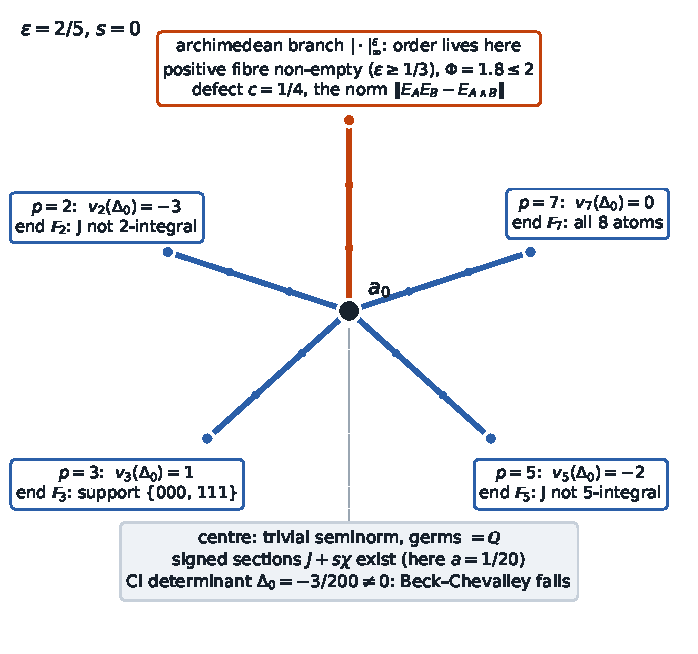
\includegraphics[width=0.84\linewidth]{fig_places}
\caption{The three-token context presheaf at $\varepsilon=\tfrac25$, read at the places of $\mathbb{Q}$ on the tree $\mathcal{M}(\mathbb{Z})$.
The centre sees the linear gluing and decides Beck--Chevalley; each finite branch sees valuations ($|\cdot|_p^\alpha$ along the branch)
and, at its end, the reduction mod $p$; only the archimedean branch carries order, positivity and the normalised defect $c$. Small dots
on a branch mark points $|\cdot|_p^{\alpha}$ for $\alpha\in(0,\infty)$. Generated by \texttt{atlas/fig\_places.py}.}
\label{fig:places}
\end{figure}

\begin{remark}[Why contexts are not separated by primes]\label{rem:places-topology}
The two windows of the Beck--Chevalley square meet only in $\sigma(X_1)$; their nerve is an edge, and the square can be drawn on two
branches through $a_0$, in the same way that the star space of \cref{sec:shadows} has one centre and many leaves. The three pair windows
of \cref{prop:three-bit} have a hollow triangle as nerve ($b_0=b_1=1$), and a tree cannot carry that cycle. Moreover, by weak
approximation the valuations of one rational law can be prescribed independently at finitely many primes, so assigning contexts to
primes imposes no gluing condition between them. Both facts point the same way as \cref{prop:places-order}: the obstruction lives in
the coefficients (positivity at $\infty$), not in the topology of $\mathcal{M}(\mathbb{Z})$. Check M8 computes the Betti numbers.
\end{remark}

\begin{remark}[Positive tropicalisation and the archimedean branch]\label{rem:places-hybrid}
The positive tropicalisation of \cref{sec:trop} needs a valuation and an order at once. Over a real closed non-Archimedean field the
order restricts to the unique ordering of $\mathbb{Q}$, which belongs to the archimedean place. So the tropical layer is not one of the
$p$-adic branches: $p$-adic valuations are blind to sign ($v_p(-x)=v_p(x)$) and allow cancellation of positive quantities
($v_3(\tfrac13)=v_3(\tfrac23)=-1$, yet the sum is $1$). It reads naturally as the degeneration $\varepsilon\to0$ of the archimedean branch,
in the sense of the hybrid spaces of Boucksom and Jonsson \cite{BoucksomJonsson2017}. We have not proved this (\cref{op:hybrid}).
\end{remark}

\begin{problem}[The tropical layer as a hybrid degeneration]\label{op:hybrid}
Realise the positive tropicalisation of \cref{sec:trop} as the restriction of the context presheaf to the end of the archimedean branch
in a hybrid analytic space over $\mathbb{Z}$, compatibly with \cref{prop:places-centre,prop:places-order,prop:places-bc}.
\end{problem}

\paragraph{An interactive view.} \Cref{fig:explorer} shows the explorer that accompanies this section and \cref{sec:halluc}
(\texttt{explorer/context\_sheaf.html}, a single page with no dependencies). It puts the six layers of the example side by side: the
contexts and their window tables, the marginal polytope, the fibre of global laws, the conditional-expectation flow with the defect
$c$ and $I(X_0;X_2\mid X_1)$, the support face, and the outcome. Check E1 reproduces its numbers at $\varepsilon=0.4$.

\begin{figure}[!htbp]\centering
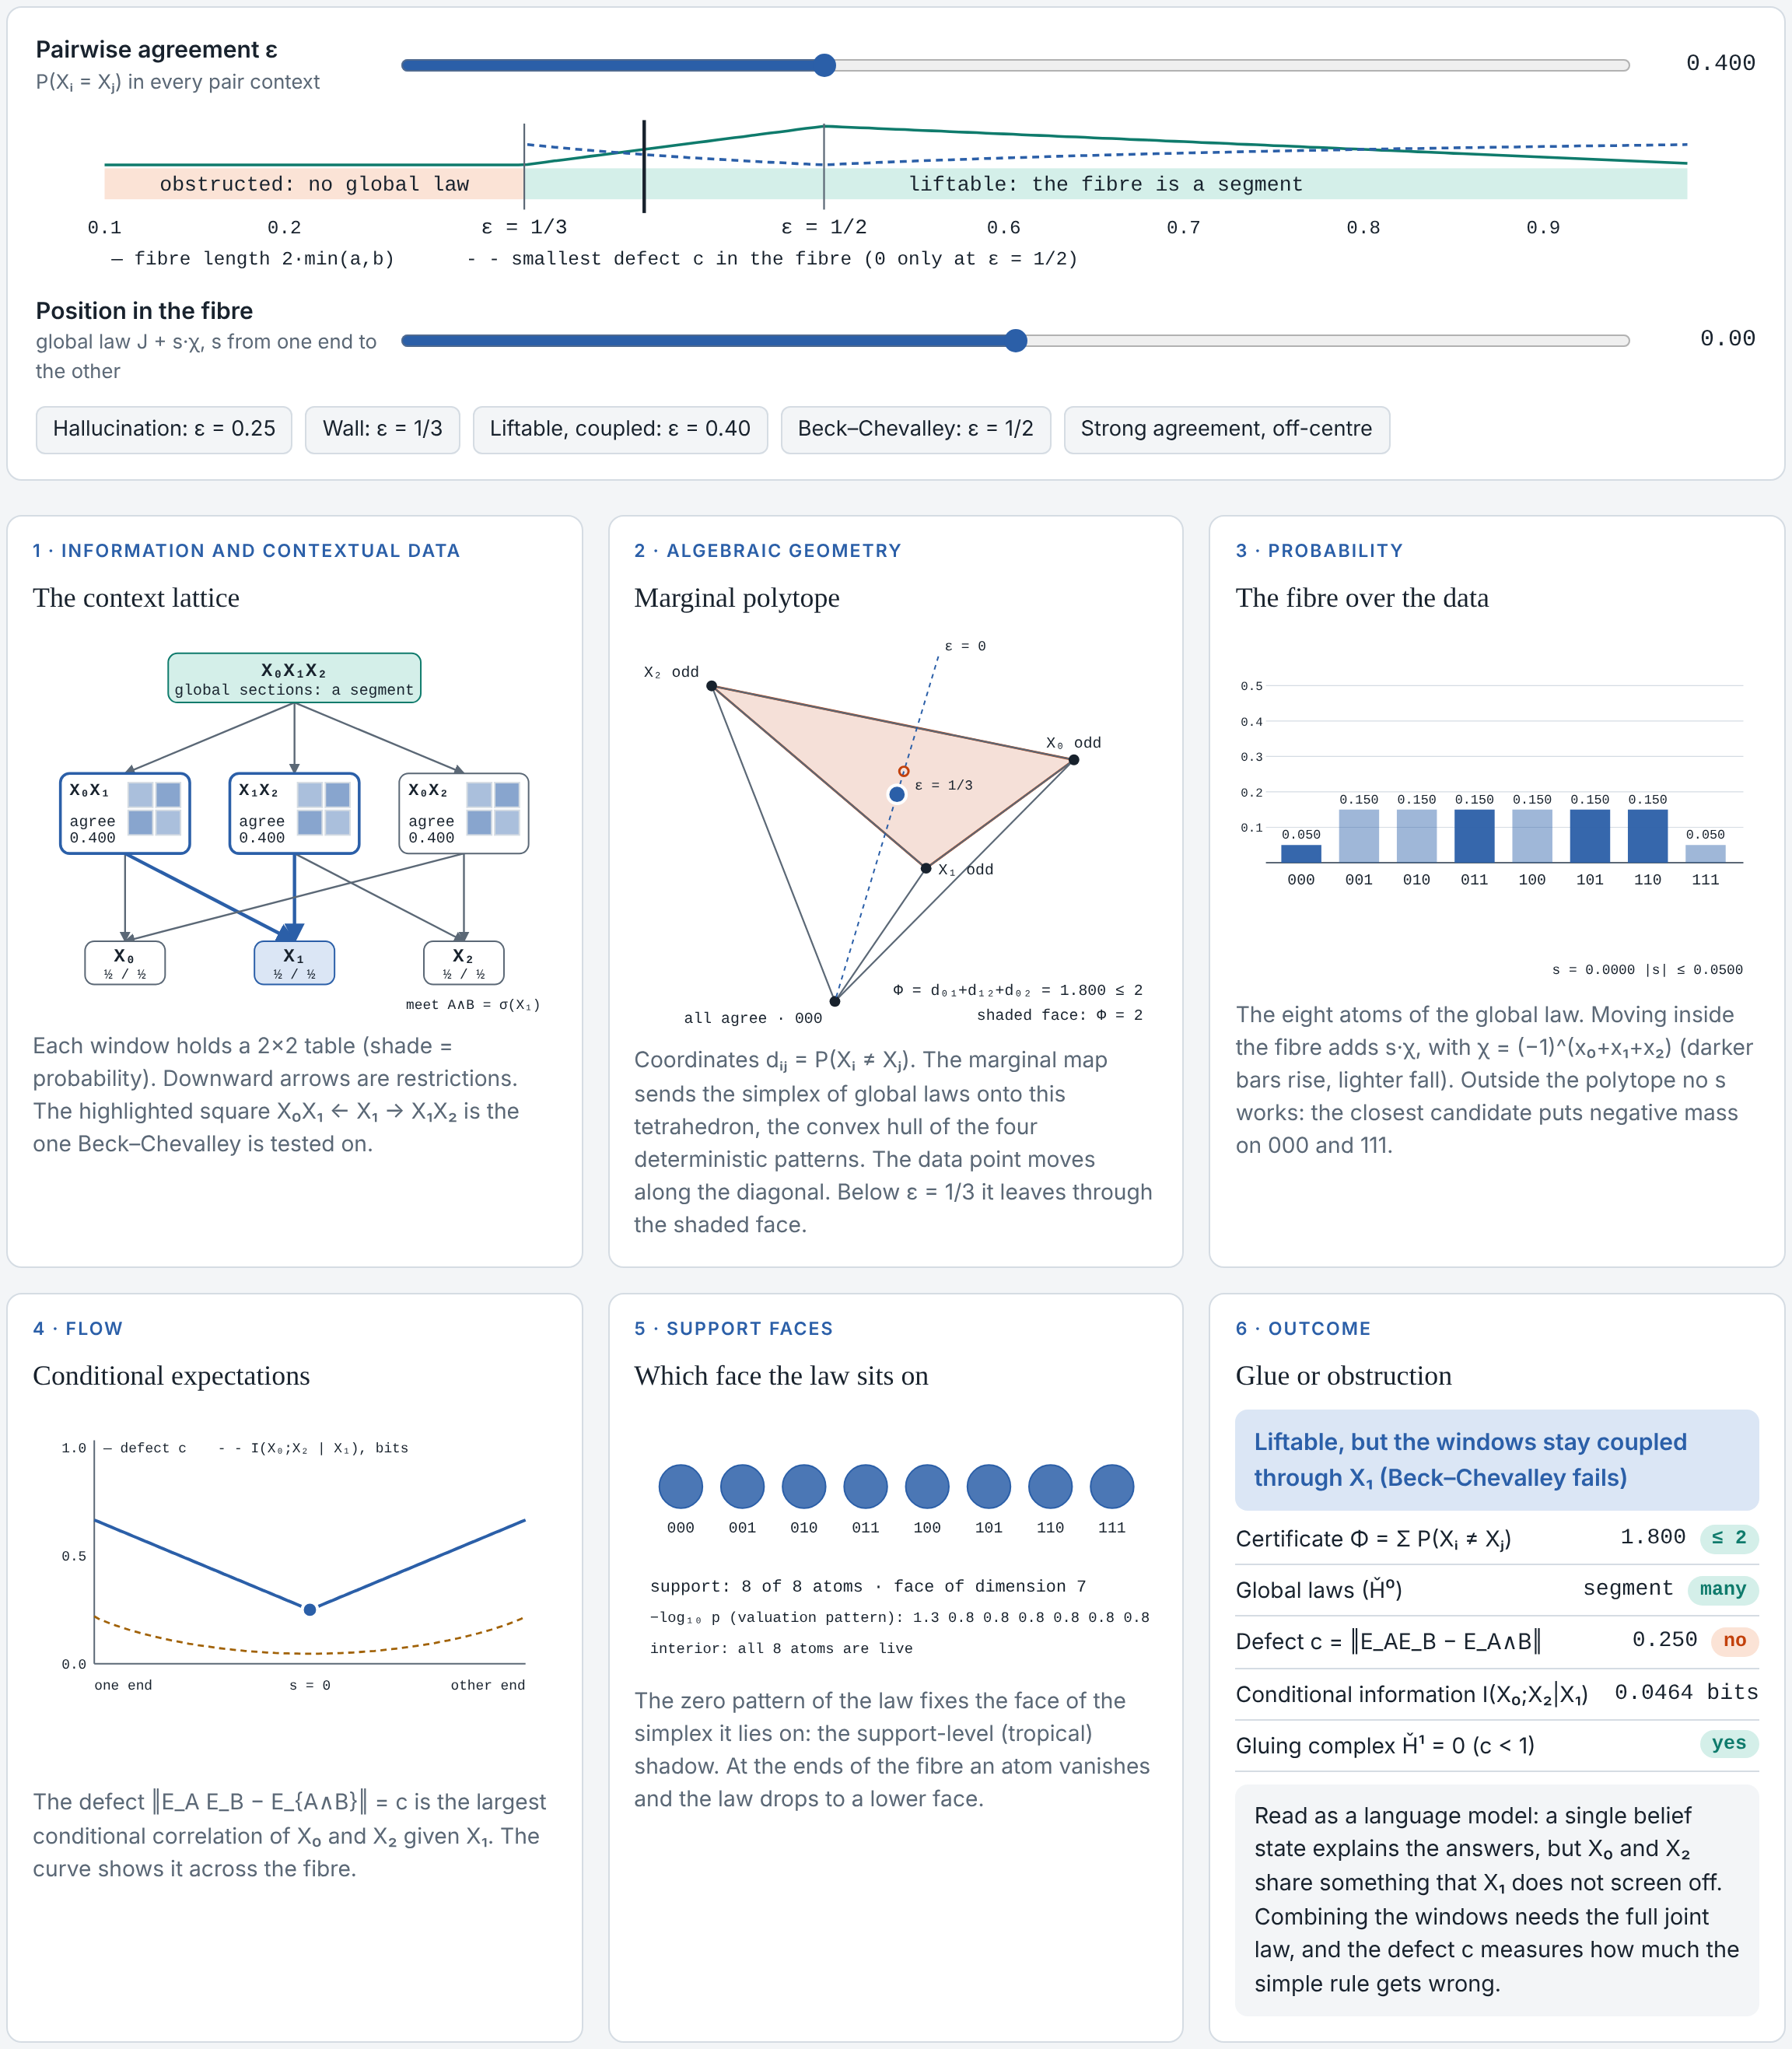
\includegraphics[width=\linewidth]{fig_explorer.png}
\caption{The explorer at $\varepsilon=0.40$, $s=0$: liftable, with $\Phi=1.8$, $c=0.25$ and $I(X_0;X_2\mid X_1)=0.0464$ bits. The phase
line shows the fibre length $2\min(a,b)$ and the smallest defect in the fibre, which is $0$ only at $\varepsilon=\tfrac12$.}
\label{fig:explorer}
\end{figure}
\FloatBarrier

%=====================================================================
\section{Three agents}\label{sec:agents}
%=====================================================================
The tower is one agent's hierarchy. This section asks what can be inferred when three agents each report a tower about the same
state, and which conclusions need joint data. Each statement is either a short derivation or a cited theorem, and
\texttt{check\_agents.py} tests the code that computes it (checks AG1--AG6).

\paragraph{Setting.} A binary state $X$ has prior $P(X=1)=\rho$. Agent $i$ sees a signal $S_i$ with kernel $P(S_i\mid X)$ and reports
the posterior $q_i=P(X=1\mid S_i)$. Agent $i$'s tower is the law $\Pi_i$ of $q_i$, with barycentre $\rho_i=\int q\,d\Pi_i$. When the
agents are pooled, the agent index $Z$ is drawn with weights $w_i$. When reports are logged, $A_i\in\{0,1\}$ is agent $i$'s binary
answer.

\begin{proposition}[Common prior]\label{prop:agents-prior}
\begin{enumerate}[label=(\alph*)]
\item If the agents are Bayesian with common prior $\rho$, then $\rho_i=\rho$ for every $i$.
\item For the pooled agents, with $\bar\rho=\sum_iw_i\rho_i$,
\[
H(\bar\rho)=\underbrace{H(\bar\rho)-\textstyle\sum_iw_iH(\rho_i)}_{I(X;Z)}+\underbrace{\textstyle\sum_iw_i\bigl(H(\rho_i)-\EE H(q_i)\bigr)}_{I(X;S_Z\mid Z)}
+\underbrace{\textstyle\sum_iw_i\,\EE H(q_i)}_{H(X\mid Z,S_Z)}.
\]
The first term vanishes iff all $\rho_i$ are equal. So $I(X;Z)$ measures how far the agents are from any common prior.
\end{enumerate}
\end{proposition}
\begin{proof}
(a) $\EE[q_i]=\EE[P(X=1\mid S_i)]=P(X=1)$; this is Bayes plausibility \cite{KamenicaGentzkow2011} and the first step of the martingale of
\cref{thm:martingale}. (b) The chain rule of mutual information along $Z$, then $S_Z$; $P(X=1\mid Z=i)=\rho_i$. Strict concavity of $H$ gives
the equality case. Checks AG1 and AG2.
\end{proof}

\begin{proposition}[Who knows more]\label{prop:agents-blackwell}
Suppose $\rho_i=\rho_j$.
\begin{enumerate}[label=(\alph*)]
\item If $S_j$ is a garbling of $S_i$ (it depends on $X$ only through $S_i$), then $\Pi_j\cx\Pi_i$.
\item Conversely, $\Pi_j\cx\Pi_i$ implies that $S_j$ is equivalent to a garbling of $S_i$ (Blackwell \cite{Blackwell1953}).
\item For a binary state, $\Pi_j\cx\Pi_i$ iff $\EE(q_j-t)_+\le\EE(q_i-t)_+$ at every support point $t$ of either law
  \cite[Thm.~3.A.1]{ShakedShanthikumar2007}. This is an exact finite test.
\item Mutual information respects the order: $\Pi_j\cx\Pi_i$ implies $I(X;q_j)\le I(X;q_i)$. The converse fails: mutual information ranks
  agents that the order leaves incomparable.
\end{enumerate}
\end{proposition}
\begin{proof}
(a) $q_j=P(X=1\mid S_j)=\EE[P(X=1\mid S_i)\mid S_j]=\EE[q_i\mid S_j]$, so $(q_j,q_i)$ is a martingale coupling. (b) is Blackwell's theorem.
(c) For laws on $[0,1]$ with equal means, convex order is the order of stop-loss transforms; these are piecewise linear with kinks at
support points. (d) $I(X;q)=H(\rho)-\EE H(q)$ and $-H$ is convex. Check AG3 confirms (a) on 150 garblings and agreement of the stop-loss test
with the martingale-coupling linear program on 300 pairs; check AG4 gives the counterexample to the converse of (d).
\end{proof}

\begin{example}[Three agents with $\rho=\tfrac12$]\label{ex:agents}
Agent $a$ has accuracy $0.8$: $\Pi_a=\tfrac12\delta_{1/5}+\tfrac12\delta_{4/5}$. Agent $b$ learns $X$ exactly with probability $0.2$ and
nothing otherwise: $\Pi_b=\tfrac1{10}\delta_0+\tfrac45\delta_{1/2}+\tfrac1{10}\delta_1$. Agent $c$ sees $a$'s signal flipped with
probability $\tfrac14$: $\Pi_c=\tfrac12\delta_{7/20}+\tfrac12\delta_{13/20}$. Then $c\prec a$ by \cref{prop:agents-blackwell}(a), and $b$ is
incomparable with both: at $t=\tfrac12$ the stop-loss of $b$ is smaller than those of $a$ and $c$, and at $t=\tfrac45$ it is larger. Mutual
information still orders them $a>b>c$ ($0.278$, $0.200$, $0.066$ bits), hiding that $b$ knows something neither of the others knows: on a
fifth of the items it is certain.
\end{example}

\begin{proposition}[Reconciling three agents]\label{prop:agents-glue}
Suppose the logs record the answers of agents $i$ and $j$ on the same items, for some pairs $\{i,j\}$, and each agent's answers are
calibrated with known accuracy. Call the logs \emph{feasible} if some common prior and private signals produce all of them.
\begin{enumerate}[label=(\alph*)]
\item If the pairs $\{1,2\}$ and $\{2,3\}$ are each feasible, they are jointly feasible. So two overlapping pairs never reveal an
  inconsistency.
\item Any feasible logs for all three pairs satisfy the cycle inequalities
  \[
  d_{ik}\le d_{ij}+d_{jk}\quad(\text{all three orders}),\qquad d_{12}+d_{23}+d_{13}\le2,\qquad d_{ij}=P(A_i\ne A_j).
  \]
  For three binary variables without calibration these four inequalities are also sufficient. With calibration the exact test is a
  linear program over $P(X,A_1,A_2,A_3)$.
\item With accuracy $\tfrac34$ for all three agents and $d_{12}=d_{23}=\tfrac1{20}$, $d_{13}=\tfrac12$, every pair is feasible and the chain
  $\{1,2\},\{2,3\}$ is feasible, but the three pairs together are not. The certificate is $d_{13}\le d_{12}+d_{23}$, violated by
  $\tfrac25$: agents 1 and 3 each nearly copy agent 2, yet agree with each other only half the time.
\end{enumerate}
\end{proposition}
\begin{proof}
(a) A feasible pair $\{i,j\}$ has a law on $(X,A_i,A_j)$. Calibration and the observed answer rates fix the $(X,A_2)$ margin, so the two
laws agree on it, and the gluing formula of \cref{prop:two-layers}(a), with $V=(X,A_2)$, gives a law on $(X,A_1,A_2,A_3)$ with both pairs
and all three calibrations. The formula needs no full-support assumption for existence (set $0/0=0$).
(b) $A_i\ne A_k$ forces $A_i\ne A_j$ or $A_j\ne A_k$; and each of the eight outcomes of $(A_1,A_2,A_3)$ has $0$ or $2$ disagreeing pairs.
These four inequalities are the facets of the cut polytope of the triangle, which proves sufficiency without calibration; the last one
is $\Phi\le2$ of \cref{prop:three-bit}.
(c) Check AG5 solves the linear programs and computes the violation exactly.
\end{proof}

\begin{proposition}[Pooling three agents]\label{prop:agents-pool}
With $X$ recorded in the logs, the chain rule
\[
\hat P(X\mid a_1,a_2,a_3)\ \propto\ \frac{P(X,a_1,a_2)\,P(X,a_2,a_3)}{P(X,a_2)}
\]
uses only the windows $\sigma(X,A_1,A_2)$ and $\sigma(X,A_2,A_3)$. It equals the true posterior when $A_1\perp A_3\mid(X,A_2)$, which for a
full-support law is Beck--Chevalley for these windows (\cref{thm:bc}). For generic laws it fails, and the defect $c$ is positive. The
familiar product of independent experts, $\hat P\propto\rho\prod_i P(a_i\mid X)$, is exact when $A_1,A_2,A_3$ are mutually independent given
$X$, which is stronger.
\end{proposition}
\begin{proof}
Under $A_1\perp A_3\mid(X,A_2)$ the joint is the glued law of \cref{prop:two-layers}(a), and conditioning on $(a_1,a_2,a_3)$ gives the
formula. Check AG6: on 200 laws built with this independence the error is below $10^{-12}$ and $c=0$; on 200 generic laws both are
positive.
\end{proof}

\paragraph{What the towers alone cannot give.} Each tower describes one agent's uncertainty about $X$. None of them says what agent $1$
believes about agent $2$. That needs agent $1$ to report a law over agent $2$'s posteriors, which is a further tower whose
``predictors'' are the other agents. The tests above then apply one level up. Without such reports, statements about beliefs about
beliefs are assumptions. Feasibility of joint posteriors for many agents is studied in \cite{ArieliEtAl2021}; for $n$ agents the cycle
inequalities remain necessary, and \cref{prop:agents-glue}(a) extends to any tree of overlapping pairs.

\FloatBarrier
%=====================================================================
\section{Empirical tests of the hallucination example}\label{sec:empirical}
%=====================================================================
The tests were pre-registered before any of the statistics below was computed, in the file \texttt{PREREG\_hallucination.md} of the folder \texttt{halluc\_study} (its
SHA-256 begins \texttt{4a34e1bb}). The same file discloses an earlier, different analysis of the same data in the validation paper.
There were three studies. Study~1 runs on public data. Study~2 was run on samples from a local model; its analysis follows a frozen
amendment. Study~3 needs pairwise elicitation from a model and ships as a kit with a synthetic smoke test.

\subsection{Why only the second layer can be tested on existing data}
The obstruction of \cref{prop:three-bit} needs each pair of tokens to be observed in a separate context. In existing benchmarks every
item's answers are observed jointly, and a jointly observed table always has a joint law, so the gap below $\tfrac13$ cannot appear in
them. Study~3 is designed to collect pairwise data. On jointly observed data the testable layer is the second one: the window
Beck--Chevalley defect of \cref{prop:windows}.

\subsection{Study 1: LLM-drift answers}
\paragraph{Data.} The data are the answers of GPT-3.5 (0301, 0613) and GPT-4 (0314, 0613) to the same items \cite{ChenZaharia2024}:
four runs per item, one answer each. Five tasks have a reference answer comparable by equality: USMLE (intact prompts), primality,
happy numbers, HotpotQA (agent) and ARC. The extraction rules are those of the validation paper, unchanged.

\paragraph{P1: consistency detector.} For a target run, the score is the fraction of the other runs whose valid answer differs from the
target's. The outcome is whether the target answer is wrong. This is the cross-sample consistency principle of SelfCheckGPT
\cite{Manakul2023}, with the other runs playing the role of samples.

\paragraph{P2: window defect.} The binary correctness of GPT-4 March, GPT-4 June and GPT-3.5 June is read through two windows:
\[
A=\sigma(Y_{\mathrm{4M}},Y_{\mathrm{4J}})\ \text{(same model, two dates)},\qquad B=\sigma(Y_{\mathrm{4J}},Y_{\mathrm{35J}})\ \text{(same date, two models)}.
\]
They share $Y_{\mathrm{4J}}$. By \cref{prop:windows}, Beck--Chevalley holds iff the March GPT-4 errors and the June GPT-3.5 errors are
independent given the June GPT-4 error. The defect $c$ is tested against a parametric Markov null.

\begin{table}[!htbp]\centering\small
\caption{Study 1 (pre-registered). AUROC of the disagreement score for target runs GPT-4 June (primary) and GPT-3.5 June (secondary),
and the window Beck--Chevalley defect $c$ with its Markov-null median and Holm-adjusted $p$-value ($B=2000$; 95\% bootstrap intervals).}
\label{tab:study1}
\resizebox{\linewidth}{!}{%
\begin{tabular}{lrrccrccc}\toprule
task & $n$ & wrong & AUROC (4J) & AUROC (35J) & $n_c$ & $c$ & null & $p_{\mathrm{Holm}}$\\\midrule
USMLE & 340 & 52 & 0.692 [0.617, 0.766] & 0.895 [0.853, 0.930] & 338 & 0.096 [0.033, 0.401] & 0.106 & 0.756\\
primes & 1000 & 489 & 0.881 [0.861, 0.901] & 0.739 [0.704, 0.771] & 949 & 0.498 [0.411, 0.584] & 0.047 & 0.003\\
happy numbers & 500 & 324 & 0.873 [0.840, 0.902] & 0.888 [0.855, 0.917] & 387 & 0.098 [0.020, 0.211] & 0.082 & 0.756\\
HotpotQA & 4844 & 2693 & 0.708 [0.694, 0.721] & 0.800 [0.783, 0.817] & 324 & 0.309 [0.128, 0.519] & 0.083 & 0.005\\
ARC & 467 & 341 & 0.821 [0.779, 0.862] & 0.902 [0.854, 0.945] & 467 & 0.320 [0.200, 0.446] & 0.069 & 0.003\\
\bottomrule
\end{tabular}}
\end{table}

\paragraph{Results.}
\begin{itemize}
\item \emph{H1 is supported.} Disagreement with the other runs detects wrong GPT-4 June answers in all five tasks, with AUROC between
  $0.69$ and $0.88$ and every interval above $0.5$.
\item \emph{H2 is supported.} Beck--Chevalley fails in three tasks: primes ($c=0.50$ against a null median of $0.05$), HotpotQA ($0.31$)
  and ARC ($0.32$). In these tasks the errors of the two outer runs stay coupled after conditioning on the shared run. By
  \cref{prop:windows}, this is coupling that neither window holds: a shared item-level difficulty that a single run does not screen
  off. In USMLE and happy numbers the defect is indistinguishable from the Markov null.
\item \emph{Exploratory.} The rank correlation between $c$ and the GPT-4 June AUROC across the five tasks is $0.70$. With five
  tasks this carries no inferential weight.
\end{itemize}

\paragraph{What Study 1 does and does not show.} It shows that the window defect is measurable on real model outputs, and that it is
nonzero in several tasks. It also replicates the consistency principle that underlies black-box hallucination detection. It does not
test the obstruction below $\tfrac13$, for the reason given above. Its errors are factual errors against a reference, a common proxy for
hallucination \cite{Ji2023} but not the same as an obstructed claim in the sense of \cite[\S10.5]{Tower}.

\subsection{Study 2: HaluEval QA}
\paragraph{Data and amendment.} HaluEval QA \cite{Li2023HaluEval} (MIT licence) gives, for each item, knowledge, a question, a right
answer and a hallucinated answer. Llama~3.1 (8B, run locally through Ollama) was sampled $K=5$ times per prompt at temperature $1$
on items $0$--$1999$, with the system line ``Answer with a short phrase only''. Items $0$--$199$ were inspected first; that inspection
found that answer length alone separates the two answer types, and that the containment judge misses paraphrases. Amendment~1
(\texttt{AMENDMENT1.md}, SHA-256 beginning \texttt{07782f4e}) was frozen after that and before any statistic on items $200$--$1999$
was computed. It adds a length baseline, a length-adjusted AUROC, a logistic test of the detector beyond length, a relaxed
deterministic judge, and a within-sample window test. Deviations from the original registration: $N=2000$ rather than $10\,000$, the
system line, and the choice of model. The confirmatory set is items $200$--$1999$ ($n=1800$).

\begin{table}[!htbp]\centering\small
\caption{Study 2, confirmatory set ($n=1800$ items, $3600$ answers; Amendment~1). Detector = fraction of the five samples that do not
match the answer. Length-adjusted AUROC compares answers only within the same length quintile. LR = likelihood-ratio statistic for
adding the detector to $\log(\text{length})$ in a logistic model. 95\% bootstrap intervals over items ($B=2000$).}
\label{tab:study2}
\begin{tabular}{lccc}\toprule
judge & AUROC & length-adjusted AUROC & LR ($p$)\\\midrule
containment (pre-registered) & 0.871 [0.860, 0.881] & 0.851 [0.827, 0.874] & 404 ($<10^{-80}$)\\
relaxed (Amendment 1)        & 0.870 [0.859, 0.882] & 0.883 [0.861, 0.903] & 493 ($<10^{-100}$)\\\midrule
length alone                 & 0.974 & --- & ---\\\bottomrule
\end{tabular}
\end{table}

\paragraph{Results.}
\begin{itemize}
\item \emph{The detector works, but length is the stronger cue in this benchmark.} The pre-registered AUROC is $0.871$. Answer length
  alone reaches $0.974$: HaluEval's hallucinated answers are usually longer than the right ones. So the raw AUROC cannot be read as
  evidence for the detector.
\item \emph{H1$''$ is supported: the detector adds information beyond length.} Within length quintiles the detector still separates the
  two answer types (AUROC $0.85$ with the containment judge, $0.88$ with the relaxed judge), and adding it to a length-only logistic
  model improves the fit by $\mathrm{LR}=404$ (cluster-robust Wald $p<10^{-80}$, allowing for the two answers per item). The
  adjustment is uneven: the middle quintile holds most of the comparisons, and in the outer quintiles one answer type has only $7$ to
  $31$ members.
\item \emph{H2$'$ is supported: the within-sample windows fail Beck--Chevalley.} Let $Y_k=1$ if sample $k$ misses the right answer
  (relaxed judge; $14.7\%$ of samples). With windows $\sigma(Y_1,Y_2)$ and $\sigma(Y_2,Y_3)$, the mass-weighted defect is
  $\bar c=0.32$ against a permutation-null median of $0.03$ ($p=0.0005$). Adding the difficulty count $D=Y_4+Y_5$ to the centre reduces
  it to $0.13$ (null $0.02$, $p=0.005$).
\end{itemize}

\paragraph{Interpretation.} The five samples are independent given the item, so the defect does not come from the sampling. It comes from
a variable missing from the lattice: the item itself. The wrong-count distribution shows this. $1441$ items have no wrong sample and
$183$ have all five wrong, against $813$ and $0$ expected under one common error rate. A model that is wrong on an item tends to be
wrong in the same way every time. One sample in the centre does not screen this off; adding two more absorbs most of it, as the
centre-enlargement reading of \cref{prop:windows} predicts. This is a common cause, not an obstruction: the samples are jointly
observed, so a joint law exists. The $183$ consistently wrong items are where a consistency detector is blind.

\paragraph{Does the test detect Beck--Chevalley correctly?} The theorem side is exact: Beck--Chevalley holds iff the outer variables are
independent given the centre (\cref{thm:bc}, checks H1, H2, L4). The finite-sample test was checked separately on synthetic data
(\texttt{check\_bc\_test.py}).
\begin{itemize}
\item \emph{When Beck--Chevalley holds it rejects at the nominal rate.} On random Markov chains $Y_1-Y_2-Y_3$ the rejection rate at
  level $0.05$ is $0.056$ ($n=300$) and $0.060$ ($n=1800$) over $1000$ replications, with uniform $p$-values. The population defect is
  $0$ for all of $200$ random Markov laws.
\item \emph{When it fails it detects it.} With item-level latent difficulty (samples i.i.d.\ given the item) the population defect is
  $0.35$. The power is $0.76$ at $n=100$ and $1.00$ from $n=300$, and the sample $\bar c$ matches the population value at every $n$.
\item \emph{Centre enlargement works as \cref{prop:windows} says.} With the latent class in the centre, Beck--Chevalley holds again and
  the rejection rate is $0.042$. The proxy $D=Y_4+Y_5$ only shrinks the defect ($0.35\to0.10$).
\item \emph{Replica of Study 2.} A three-class binomial model fitted to the wrong-count distribution alone gives simulated $\bar c$
  intervals $[0.30,0.56]$ (centre $Y_2$) and $[0.07,0.41]$ (centre $(Y_2,D)$). Both contain the observed values $0.32$ and $0.13$. This
  model has as many parameters as free cells, so the replica shows consistency, not a test of the latent reading.
\end{itemize}

\paragraph{Limitations.} Both judges are string-based. The relaxed judge still misses name variants (``Don Henley'' against ``Donald
Hugh Henley''), which inflates the detector score of some right answers. A meaning-based judge is the next step. HaluEval's
hallucinated answers were written to a template, which produces the length gap; the length-adjusted results are the ones to cite.

\subsection{Study 3: kit}
\begin{itemize}
\item \emph{Study 3} (\texttt{kit\_pairwise\_cycles.py}) asks about each pair of three related claims in a separate prompt, and
  evaluates the 3-cycle inequalities of \cite[Thm.~4.8]{Conditionals}. It reports the largest violation $V$ with a bootstrap interval.
  For the symmetric model $V=2(1-3\varepsilon)$; the smoke test recovers $V\approx0.5$ at $\varepsilon=0.25$ and no violation at
  $\varepsilon=0.45$. This is the design in which a hallucination in the sense of \cref{prop:three-bit} can be observed directly.
\end{itemize}
TruthfulQA \cite{Lin2022TruthfulQA} can supply claim triples for Study~3 once model answers are collected.

\FloatBarrier
%=====================================================================
\section{Computational checks}\label{sec:checks}
%=====================================================================

\subsection{The scripts}
\begin{itemize}
\item \texttt{check\_shadows.py} has 30 checks, in exact rational arithmetic except A1(v) and A4, which use double precision with
  tolerance $10^{-9}$. It imports the tower objects from \texttt{check\_tower.py}.
\item \texttt{check\_tropical.py} has 8 checks, in exact Puiseux arithmetic except the floating-point ranks in T6 and T7.
\item \texttt{check\_cohomology.py} has 10 checks, exact except H2.
\item \texttt{check\_hallucination.py} has 9 checks, exact except L4b, L5 and L7.
\item \texttt{check\_agents.py} has 6 checks (AG1--AG6) of \cref{sec:agents}, exact except the information quantities and linear programs.
\item \texttt{check\_barr.py} has 4 checks (R1--R4) of \cref{lem:barr}, by linear-programming feasibility on random instances, with negative controls and a counterexample to the converse of (d).
\item \texttt{check\_places.py} has 9 checks (M1--M8, E1), exact except the floating-point $I$ in E1.
\item \texttt{check\_bc\_test.py} has 7 Monte Carlo checks (S1--S6) of the finite-sample Beck--Chevalley test of \cref{sec:empirical}.
\item In the folder \texttt{halluc\_study}, \texttt{study1\_llmdrift.py} runs the pre-registered Study~1 (\cref{tab:study1}), and
  \texttt{kit\_halueval.py} and \texttt{kit\_pairwise\_cycles.py} are the kits for Studies~2 and~3, with smoke tests.
\item \texttt{atlas/fig\_places.py} draws \cref{fig:places}; \texttt{explorer/context\_sheaf.html} is the explorer of \cref{fig:explorer}.
\item \texttt{atlas/atlas.py} draws \cref{fig:algebra,fig:tower,fig:secant,fig:tropical,fig:walls,fig:fibres,fig:betti,fig:hallucination}, and
  \texttt{atlas/fibre\_scan.py} computes the Betti map. Both use \texttt{atlas/fibre\_topology.py}.
\end{itemize}
All checks pass; the hashes are in \texttt{FROZEN.txt}.

\begin{center}\small
\begin{tabular}{>{\raggedright}p{1.7cm}>{\raggedright\arraybackslash}p{12.6cm}}\toprule
A1--A7b & \cref{thm:commute} (449 commuting, 151 non-commuting); \cref{prop:join}; \cref{ex:46}; \cref{thm:rate}; \cref{cor:lax};
  \cref{lem:smallC}; \cref{prop:gauss}\\
B1--B7 & star space; \cref{thm:band}; \cref{prop:no-centre}; \cref{thm:martingale}; \cref{prop:absorb};
  \cref{prop:two-idempotents,prop:fibre}; \cref{prop:beck-located}\\
C1--C7 & audit of earlier scripts; \cref{prop:naive}; \cref{ex:threshold}; \cref{prop:continuity}(b)\\
D1--D2, E1--E2 & \cref{prop:moments}; \cref{thm:T}\\
G1--G3 & \cref{prop:fusion}; \cref{prop:naturality}; \cref{prop:star-functor}\\
T1--T8 & \cref{thm:monad}; \cref{thm:lift}; \cref{thm:berk}(a); \cref{prop:posterior}; \cref{ex:dims}; \cref{prop:walls}(a)\\
H1--H5 & \cref{thm:bc}; \cref{thm:gluing}(b, d); \cref{prop:not-iso}\\
K1--K5 & \cref{thm:nerve,thm:hw-topology}; \cref{prop:local-lifts}(b); \cref{fig:betti}\\
L1--L8 & \cref{prop:three-bit,prop:windows,prop:halluc-trop}; the token stream of \cref{fig:hallucination}\\
R1--R4 & \cref{lem:barr}\\
AG1--AG6 & \cref{prop:agents-prior,prop:agents-blackwell,prop:agents-glue,prop:agents-pool}; \cref{ex:agents}\\
M1--M8, E1 & \cref{prop:places-centre,prop:places-order,prop:places-bc}; \cref{rem:places-topology}; \cref{fig:places,fig:explorer}\\
S1--S6 & the permutation test of \cref{sec:empirical}: size, power, centre enlargement, replica of \cref{tab:study2}\\
\bottomrule
\end{tabular}
\end{center}

\subsection{What checks establish}
Finite exact checks verify identities on the enumerated inputs and can falsify overbroad claims. They do not prove identities for all
measures, establish measurability, or supply categorical typing. Every general statement in this paper has a proof; the checks guard
the proofs against slips. Hashes certify the identity of artefacts, not the truth of theorems.

\subsection{Audit of earlier scripts}
Five scripts accompanied an earlier version. All five share one nearest-atom \texttt{pooling(nu, atoms)}, with ``type-aware'' total
variation and ties broken by key order. They pass every reported check for the following reasons:
\begin{longtable}{>{\raggedright}p{3.7cm}>{\raggedright\arraybackslash}p{11cm}}
\toprule Script & Why it passes\\\midrule\endfirsthead\toprule Script & Why it passes\\\midrule\endhead
\texttt{check\_giry.py} & $\Pi$ always has two atoms, and $\Sigma$'s descriptors $i\bmod2$ biject with them. So $\sigma(\theta)=\sigma(\rr)$,
  and $L$ and $R$ have identical cells (C1).\\
\texttt{check\_3cat\-Coherence.py} & As above. In addition, level-5 atoms of type $\D^2$ against inputs of type $\D^1$ are all at TV
  distance $1$, so the pooling is total, $\ebot$, and the ``3-cell'' is trivial (C7).\\
\texttt{check\_non\-coherent.py} & The duplicated predictive $(0,\rho_1),(1,\rho_1)$ ties, and the first key wins, so $R$'s cells equal
  $L$'s (C6).\\
\texttt{double\_\-category.py} & ``Interchange'' is $R(L\nu)=L(R\nu)$ with $L=R$. ``(U) defect nonzero'' is $\ebot\ne\etop$.\\
\texttt{check\_span.py} & The cells coincide (C1). \texttt{dist\_of} strips $\theta$, so ``not inverse'' holds by a change of key type.
  ``(Cm) equals sum'' compares a pair with itself (C5). Mixed inputs combine two key types under one metric.\\
\bottomrule
\end{longtable}
By \cref{prop:naive}, any composite of nearest-atom poolings is one pooling onto a coarsening of the first partition. By
\cref{prop:posterior}, such pooling is a zero-temperature shadow. The scripts' counts therefore carry no information about
\cref{thm:commute}. A meaningful test uses the star space with labels that are not functions of the predictive, and compares three
pairs: canonical shadows, label-only shadows, and naive composites. Checks B2, B3 and C2 do exactly this.

%=====================================================================
\section{Consequence for the tower paper}\label{sec:tower-remark}
%=====================================================================
The tower paper \cite{Tower} never uses $E_BE_A=E_{A\vee B}$. Its poolings live on a fixed sample index \cite[Def.~13.13]{Tower}, and
its order in \cite[Thm.~13.16]{Tower} is a transitive closure. An unnumbered paragraph added after that theorem explains why the
closure is needed. A two-step label pooling $E_{G_2}E_{G_1}$ is one conditional expectation iff the two commute, which by
\cref{thm:commute} means conditional independence given $G_1\wedge G_2$; the product is then $E_{G_1\wedge G_2}$, never the join.

%=====================================================================
\section{Summary and open problems}
%=====================================================================
\begin{itemize}
\item Two conditional expectations commute iff they are conditionally independent given their meet. Otherwise they interchange laxly,
  through the meet, at the exact rate $c^{2n-1}$. The join identity is false except for equal $\sigma$-algebras.
\item The canonical shadows of a context live on its star space. They form a commutative band, are natural along context maps that are
  injective on predictive atoms, and interchange strictly.
\item The tower acts on barycentre fibres as a martingale. $\ebot$ and $\etop$ are the bottom and top of each fibre. Each computed Beck
  defect is one conditional-expectation step.
\item Over a real non-Archimedean field the whole picture tropicalises exactly: the valuation is a monad morphism, fibres lift,
  mixtures become tropical secants, and the valuation factors through Berkovich spaces. Hard assignment is the zero-temperature
  shadow.
\item Conditional expectation is restriction in the $L^2$ presheaf. Commutation is its Beck--Chevalley condition, and gluing fails only
  when $c=1$. Tropical fibres have computable cohomology, read off from certificates of impossible assignment patterns. In the
  Hardy--Weinberg example the collision wall is a jump $\Delta b_0=-1$.
\item In a three-token model a hallucination is a failure to glue pairwise windows, certified by a Bell-type functional, below a
  straight wall in source weights. Two windows always glue, so failure needs a cycle in the cover; the Beck--Chevalley defect is a
  separate layer and stays at $\tfrac12$ at the wall.
\item For three agents, convex order of their towers is Blackwell's information order, which mutual information totalises; the
  agent-level entropy term vanishes iff they share a prior; two overlapping pairs of logs always reconcile, three can fail with a cycle
  certificate; and chain pooling is exact under Beck--Chevalley. Above the wall, overlapping windows commute iff the tokens are Markov through the shared token. The
  Friedrichs cosine is the exact measure of the coupling that no window holds.
\item Over $\mathcal{M}(\mathbb{Z})$ the gluing problem splits by place. The linear part glues everywhere, Beck--Chevalley is decided
  at the trivial seminorm, finite places measure the defect by valuations, and positivity, hence the hallucination obstruction, lives
  only at the archimedean place.
\end{itemize}
The open problems are \cref{op:twocat,op:general,op:ident,op:order,op:cech,op:hybrid}, and \cref{conj:wall}.

\appendix
%=====================================================================
\section{Changes from the previous versions}\label{app:changes}
%=====================================================================
This paper supersedes three manuscripts of October 2026:
\begin{enumerate}[label=(\roman*)]
\item \emph{Conditional Expectations, Beck Defects, and a Proposed Double-Category Structure}, referred to below as G;
\item \emph{Conditional Expectations, Beck Defects, and the Shadow Algebra of the Posterior Tower}, referred to below as S;
\item \emph{From Barycentre Fibres to Secant Geometry}.
\end{enumerate}
S and (iii) are absorbed in full. The table lists every statement of G that changed.

\begin{longtable}{>{\raggedright}p{4.4cm}>{\raggedright}p{2.2cm}>{\raggedright\arraybackslash}p{7.8cm}}
\toprule G & Status & Here\\\midrule\endfirsthead\toprule G & Status & Here\\\midrule\endhead
Def 3.2, Props 3.3, 3.5 (label shadows) & kept & \cref{prop:label-props}; composites in \cref{prop:naive}\\
Thm 4.2 (nested) & kept & special case of \cref{thm:commute}\\
Thm 4.4 (CI $\Rightarrow$ commute) & strengthened & five-way equivalence, \cref{thm:commute}\\
Rem 4.5 (join), Ex 4.6 & kept, sharpened & \cref{prop:join}; \cref{ex:46}\\
Rem 4.7 (``hypotheses necessary'') & made precise & \cref{thm:commute}; general case \cref{thm:rate,cor:lax}\\
Prop 4.8, Rem 4.9, Prop 8.1 (inheritance) & discharged & \cref{prop:law-functor}\\
Defs 5.1, 5.3, Rem 5.4, Defs 5.5, 5.6, Props 5.7, 5.8, Rem 5.9 & kept & \cref{sec:category}; context maps defined concretely in \cref{def:ctx}\\
Def 5.10, Prop 5.11 (compatible subcategory) & proved & \cref{prop:naturality,prop:star-functor}\\
Diagram after Def 5.13 & withdrawn & horizontal composition of contexts is not a functor $\Ctx\times\Ctx\to\Ctx$\\
Thm 5.14 (interchange blueprint) & replaced & \cref{prop:quintets}\\
Prop 6.1 (required data) & kept & \cref{prop:required}, now supplied by \cref{prop:single-step}\\
Conj 6.2 (two-shadow factorisation) & superseded & one step suffices in every computed case\\
Thms 7.1, 7.2 (Options A, B) & partly invalid & \cref{prop:options}: (Cm) does not decompose\\
\S8 (Giry) & completed & \cref{sec:giry}\\
Prop 9.1, Rem 9.2 (3-cells) & kept & triviality in quintets\\
\S10 (regimes) & kept & worked regimes in \cref{sec:algebra}\\
Def 11.1, Thms 11.2, 11.5 (double category of the tower) & withdrawn & 2-cells mistyped; \cref{prop:quintets}\\
Thm 11.4, Prop 11.8 & kept & identities and latent relabellings are natural (\cref{sec:gauss})\\
Prop 11.7 (Gaussian interchange) & false & \cref{prop:gauss}\\
\S11.6.1 (restricted domain $V$) & corrected & the square is total (\cref{sec:gauss})\\
\S12 (scope of checks) & kept & \cref{sec:checks}\\
\S13 (Berkovich programme) & replaced & \cref{sec:trop}\\
\S14 (stochastic-to-convex bridge) & kept, strengthened & \cref{thm:T}: fully faithful; shadows not affine\\
\S15 (Wasserstein--Berkovich functor) & withdrawn & ill-defined; \cref{thm:berk} instead\\
\S16 (secants, wall-crossing) & corrected & \cref{sec:secant}: order $\ge3$; hierarchy invisible to moments; \cref{conj:wall}\\
\bottomrule
\end{longtable}

\section*{Code and data availability}
\addcontentsline{toc}{section}{Code and data availability}
All scripts, figure generators, the interactive explorer, the pre-registration and its amendment, and the study kits are at
\url{https://github.com/vkawasth/Trainingless-Transformer-NoGradientDescent/tree/main/papers}. The HaluEval and LLM-drift data are
downloaded from their original sources; the Study~2 samples (model outputs on HaluEval prompts) are included.

\section*{Acknowledgements}
\addcontentsline{toc}{section}{Acknowledgements}
We thank the people who collected and released the data and software used here:
\begin{itemize}[leftmargin=*,nosep]
\item L.~Chen, M.~Zaharia and J.~Zou for the LLM-drift answers \cite{ChenZaharia2024};
\item J.~Li, X.~Cheng, W.~X.~Zhao, J.-Y.~Nie and J.-R.~Wen (RUCAIBox) for HaluEval \cite{Li2023HaluEval}, released under the MIT licence;
\item S.~Lin, J.~Hilton and O.~Evans for TruthfulQA \cite{Lin2022TruthfulQA};
\item the developers of Python, NumPy, SciPy (including the HiGHS solver), SymPy, pandas and Matplotlib, on which every computation and
  figure depends.
\end{itemize}
The data are used under their licences and terms; no credentialed or patient-level data were used. The study in \cref{sec:empirical}
was pre-registered and frozen by hash before its statistics were computed. Independent reviews by language-model referees found errors
in earlier drafts of this material, which are corrected here, and an AI assistant (Claude, Anthropic) helped draft text, write the
exact-arithmetic checks and produce the figures. The author is responsible for all remaining errors.

\begin{thebibliography}{99}\small
\bibitem{Tower} V.~K. Awasthi, The three-level posterior tower: hierarchical Bayesian inference and mixed distributive laws. Technical
report, October 2026 (version 10).
\bibitem{Conditionals} V.~K. Awasthi, Conditionals, couplings and toric geometry. Technical report, October 2026.
\bibitem{PoolingNote} V.~K. Awasthi, Pooling idempotents and the Beck defects of the absolute tower. Note, October 2026.
\bibitem{AbramskyBrandenburger2011} S.~Abramsky and A.~Brandenburger, The sheaf-theoretic structure of non-locality and contextuality.
\emph{New J. Phys.} \textbf{13} (2011), 113036.
\bibitem{ChenZaharia2024} L.~Chen, M.~Zaharia and J.~Zou, How is ChatGPT's behavior changing over time? \emph{Harvard Data Science
Review} \textbf{6} (2024), no.~2; arXiv:2307.09009. Data: \url{https://github.com/lchen001/LLMDrift}.
\bibitem{Ji2023} Z.~Ji, N.~Lee, R.~Frieske, T.~Yu, D.~Su, Y.~Xu, E.~Ishii, Y.~J. Bang, A.~Madotto and P.~Fung, Survey of hallucination in
natural language generation. \emph{ACM Comput. Surv.} \textbf{55} (2023), no.~12, Article 248.
\bibitem{Li2023HaluEval} J.~Li, X.~Cheng, W.~X. Zhao, J.-Y. Nie and J.-R. Wen, HaluEval: a large-scale hallucination evaluation benchmark
for large language models. In \emph{Proc. EMNLP} (2023), 6449--6464. Data: \url{https://github.com/RUCAIBox/HaluEval}.
\bibitem{Lin2022TruthfulQA} S.~Lin, J.~Hilton and O.~Evans, TruthfulQA: measuring how models mimic human falsehoods. In \emph{Proc. ACL}
(2022), 3214--3252.
\bibitem{Manakul2023} P.~Manakul, A.~Liusie and M.~J.~F. Gales, SelfCheckGPT: zero-resource black-box hallucination detection for
generative large language models. In \emph{Proc. EMNLP} (2023), 9004--9017.
\bibitem{AFS2016} C.~Am\'endola, J.-C. Faug\`ere and B.~Sturmfels, Moment varieties of Gaussian mixtures. \emph{J. Algebr. Stat.}
\textbf{7} (2016), 14--28.
\bibitem{Alessandrini2013} D.~Alessandrini, Logarithmic limit sets of real semi-algebraic sets. \emph{Adv. Geom.} \textbf{13} (2013),
155--190.
\bibitem{BauschkeDeutschHundal2009} H.~H. Bauschke, F.~Deutsch and H.~Hundal, Characterizing arbitrarily slow convergence in the method
of alternating projections. \emph{Int. Trans. Oper. Res.} \textbf{16} (2009), 413--425.
\bibitem{Poineau2010} J.~Poineau, \emph{La droite de Berkovich sur $\mathbb{Z}$}. Ast\'erisque \textbf{334}, Soc. Math. France, 2010.
\bibitem{BoucksomJonsson2017} S.~Boucksom and M.~Jonsson, Tropical and non-Archimedean limits of degenerating families of volume forms.
  \emph{J. \'Ec. polytech. Math.} \textbf{4} (2017), 87--139.
\bibitem{Vorobev1962} N.~N. Vorob'ev, Consistent families of measures and their extensions. \emph{Theory Probab. Appl.} \textbf{7}
  (1962), 147--163.
\bibitem{Serre1973} J.-P. Serre, \emph{A Course in Arithmetic}. Graduate Texts in Mathematics 7, Springer, 1973.
\bibitem{Barr1970} M.~Barr, Relational algebras. In \emph{Reports of the Midwest Category Seminar IV}, LNM 137, Springer, 1970, 39--55.
\bibitem{Blackwell1953} D.~Blackwell, Equivalent comparisons of experiments. \emph{Ann. Math. Statist.} \textbf{24} (1953), 265--272.
\bibitem{KamenicaGentzkow2011} E.~Kamenica and M.~Gentzkow, Bayesian persuasion. \emph{Amer. Econ. Rev.} \textbf{101} (2011), 2590--2615.
\bibitem{ArieliEtAl2021} I.~Arieli, Y.~Babichenko, F.~Sandomirskiy and O.~Tamuz, Feasible joint posterior beliefs. \emph{J. Polit. Econ.}
  \textbf{129} (2021).
\bibitem{ShakedShanthikumar2007} M.~Shaked and J.~G. Shanthikumar, \emph{Stochastic Orders}. Springer, 2007.
\bibitem{Berkovich1990} V.~G. Berkovich, \emph{Spectral Theory and Analytic Geometry over Non-Archimedean Fields}. AMS, 1990.
\bibitem{Develin2006} M.~Develin, Tropical secant varieties of linear spaces. \emph{Discrete Comput. Geom.} \textbf{35} (2006), 117--129.
\bibitem{DevelinSantosSturmfels2005} M.~Develin, F.~Santos and B.~Sturmfels, On the rank of a tropical matrix. In \emph{Combinatorial and
Computational Geometry}, MSRI Publ. 52, 2005, 213--242.
\bibitem{Draisma2008} J.~Draisma, A tropical approach to secant dimensions. \emph{J. Pure Appl. Algebra} \textbf{212} (2008), 349--363.
\bibitem{Ehresmann1963} C.~Ehresmann, Cat\'egories structur\'ees. \emph{Ann. Sci. \'Ec. Norm. Sup.} \textbf{80} (1963), 349--426.
\bibitem{Giry1982} M.~Giry, A categorical approach to probability theory. LNM 915, Springer, 1982, 68--85.
\bibitem{Grandis2019} M.~Grandis, \emph{Higher Dimensional Categories: From Double to Multiple Categories}. World Scientific, 2019.
\bibitem{JellScheidererYu2022} P.~Jell, C.~Scheiderer and J.~Yu, Real tropicalization and analytification of semialgebraic sets.
\emph{Int. Math. Res. Not.} (2022), 928--958.
\bibitem{KayalarWeinert1988} S.~Kayalar and H.~L. Weinert, Error bounds for the method of alternating projections. \emph{Math. Control
Signals Systems} \textbf{1} (1988), 43--59.
\bibitem{KulisJordan2012} B.~Kulis and M.~I. Jordan, Revisiting $k$-means: new algorithms via Bayesian nonparametrics. \emph{ICML} 2012.
\bibitem{Bjorner1995} A.~Bj\"orner, Topological methods. In \emph{Handbook of Combinatorics}, Vol.~II, Elsevier, 1995, 1819--1872.
\bibitem{Deutsch2001} F.~Deutsch, \emph{Best Approximation in Inner Product Spaces}. CMS Books in Mathematics, Springer, 2001.
\bibitem{Schrijver1986} A.~Schrijver, \emph{Theory of Linear and Integer Programming}. Wiley, 1986.
\bibitem{Payne2009} S.~Payne, Analytification is the limit of all tropicalizations. \emph{Math. Res. Lett.} \textbf{16} (2009), 543--556.
\bibitem{Phelps2001} R.~R. Phelps, \emph{Lectures on Choquet's Theorem}, 2nd ed. LNM 1757, Springer, 2001.
\bibitem{Strassen1965} V.~Strassen, The existence of probability measures with given marginals. \emph{Ann. Math. Statist.} \textbf{36}
(1965), 423--439.
\bibitem{vonNeumann1950} J.~von Neumann, \emph{Functional Operators, Vol.~II}. Princeton University Press, 1950.
\end{thebibliography}
\end{document}
